\documentclass[11pt,a4paper]{article}
\usepackage[T1]{fontenc}
\usepackage[utf8]{inputenc}
\usepackage{lmodern}
\usepackage{textcomp}
\usepackage{amsmath,amssymb}
\usepackage[a4paper,margin=25mm]{geometry}
\usepackage{microtype}
\usepackage{graphicx}
\usepackage{longtable,booktabs,array,calc}
\usepackage{xcolor}
\usepackage{etoolbox}
\usepackage{newunicodechar}
\usepackage[hidelinks]{hyperref}
\usepackage{xurl}
\usepackage{parskip}
\setcounter{secnumdepth}{1}
\providecommand{\tightlist}{\setlength{\itemsep}{0pt}\setlength{\parskip}{0pt}}
\providecommand{\real}[1]{#1}
% symbols written directly in the source
\newunicodechar{≤}{\ensuremath{\le}}
\newunicodechar{≥}{\ensuremath{\ge}}
\newunicodechar{×}{\ensuremath{\times}}
\newunicodechar{·}{\ensuremath{\cdot}}
\newunicodechar{→}{\ensuremath{\to}}
\newunicodechar{−}{\ensuremath{-}}
\newunicodechar{±}{\ensuremath{\pm}}
\newunicodechar{≈}{\ensuremath{\approx}}
\newunicodechar{α}{\ensuremath{\alpha}}
\newunicodechar{β}{\ensuremath{\beta}}
\newunicodechar{Δ}{\ensuremath{\Delta}}
\newunicodechar{∏}{\ensuremath{\prod}}
\newunicodechar{⟨}{\ensuremath{\langle}}
\newunicodechar{⟩}{\ensuremath{\rangle}}
\newunicodechar{′}{\ensuremath{'}}
\newunicodechar{µ}{\textmu}
\newunicodechar{°}{\textdegree}
\renewcommand{\arraystretch}{1.15}
\setlength{\LTpre}{6pt}\setlength{\LTpost}{6pt}
\AtBeginEnvironment{longtable}{\small}
\title{AI in Mathematics, Measured: The Lean Studies}
\author{Vincent Weinreich}
\date{October 2026}

\begin{document}
\maketitle
\begin{center}\small \textcopyright{} 2026 Vincent Weinreich. Licensed under \href{https://creativecommons.org/licenses/by/4.0/}{CC BY 4.0}.\end{center}

\begin{abstract}
\noindent\emph{This edition contains the studies on Lean, mathlib and AI theorem provers.}

In pre-registered studies run between 22 September and 19 October 2026, an AI research agent measured how formal mathematics and AI theorem provers behave in Lean, and built working tools and machine-checked artefacts. Every confirmatory test was fixed in writing, with a SHA-256 hash, before any result was seen, and most pipelines were first run on synthetic data with a known answer.

\begin{itemize}
\tightlist
\item
  \textbf{Formal libraries grow like classic networks.} In mathlib, Metamath and the Archive of Formal Proofs, a lemma (in the AFP, a theory) gains new users in proportion to its current users (exponent 1.00--1.03). Refactoring removes cross-area dependencies 1.7--2.9 times as often as internal ones, a pattern four Python projects share.
\item
  \textbf{AI provers fall back on popular lemmas when they lack the specific one.} Filling a lemma gap in new mathlib proofs, two open provers chose lemmas 3.2 and 4.6 times as widely used as the human\textquotesingle s (geometric mean). Only 15 of the first prover\textquotesingle s 305 substitutes type-check.
\item
  \textbf{A symbolic layer repairs much of this.} Candidates from Lean\textquotesingle s search, model samples, text retrieval and the citation graph, ranked with a popularity correction and checked by Lean, fill 54.1 \% of held-out gaps against 11.8 \% for free generation, and 45.8 \% against 15.0 \% in theorems newer than the prover. Given to Claude Opus 5.5 without the surrounding file, the layer raised its solved theorems that need a new lemma from 79 \% to 93 \%.
\item
  \textbf{Whole proofs: Lean\textquotesingle s error messages are the lever.} About ten ways of helping a 7B prover with whole proofs all failed. Claude Opus proved 229 of 233 fresh mathlib theorems with up to three repairs from Lean\textquotesingle s errors, against 204 with four fresh attempts; GPT-6 Astra 118 of 187 against 47. Repair needs a minimum model strength (success per round 5 \% for Haiku, 60 \% for Sonnet, 72 \% for Opus), and about two thirds of its gain comes from the content of the messages.
\item
  \textbf{An open Lean model.} Leanstral 1.5 solved 66 of 95 fresh theorems as an agent, below Opus without tools (78). It finds the lemmas it needs but fails to assemble proofs; five pre-registered interventions did not help.
\item
  \textbf{Detection and audits.} At corpus level AI-written proofs are hard to recognise, but on the same theorem Claude\textquotesingle s proof is the more predictable one in 102 of 121 pairs. An AI audit found two statements in formal-conjectures listed as open that are false as formalised, one of them known since 1965.
\item
  \textbf{Verified computation.} In Lean 4 we proved 20 ≤ God\textquotesingle s number ≤ 28 for Rubik\textquotesingle s cube and at least 22 for the supercube.
\end{itemize}

The main lesson concerns method. Self-tests caught several of our own errors, one of them only after it had been reported. The costliest mistakes were checks that failed silently, a leak in our own sandbox, optimistic advance estimates, and literature searches made after a study instead of before it.
\end{abstract}

\section{Introduction}

AI systems now take part in mathematical research, but what they add is hard to judge from demonstrations. We measured it instead, in small studies whose hypotheses, tests and stop rules were fixed in advance.

Two questions guided the work:

\begin{enumerate}
\def\labelenumi{\arabic{enumi}.}
\tightlist
\item
  \textbf{How do AI provers behave on new formal mathematics?} Which lemmas do they choose, where do their proofs fail, can a cheap symbolic layer repair the failures, and can their proofs be recognised?
\item
  \textbf{What can an AI research agent achieve under strict rules?} Within four weeks, can it produce verified artefacts and establish empirical facts that hold up?
\end{enumerate}

The agent was Claude (Anthropic), working in the Cowork app. It drafted the pre-registrations, wrote and ran code in a cloud container and on the author\textquotesingle s laptop (Apple M4, 16 GB), and wrote first reports. The author set directions, contributed several study ideas and applied one standing rule: a line of work ends when nothing groundbreaking is in sight.

Besides two small open provers, the studies tested Claude Opus 5.5, Sonnet 5.5 and Haiku 4.5 through Anthropic\textquotesingle s API, GPT-6 Astra through OpenAI\textquotesingle s Codex command line and Mistral\textquotesingle s open Lean model Leanstral 1.5.

\textbf{Related work.}

\begin{itemize}
\tightlist
\item
  AlphaEvolve was applied to 67 problems; it mostly matched the best known constructions and improved several (Georgiev et al. 2025).
\item
  Gemini was run on 700 open Erdős problems; 13 were addressed, of which 4 were possibly new (2 of them partial solutions), and checking novelty was the hardest step (Feng et al. 2026).
\item
  OpenAI released formalised research results with Lean proofs on 6 October 2026 (\nolinkurl{github.com/openai/math}). We audited parts of this release (Section 7).
\item
  Open prover models such as DeepSeek-Prover-V2 and Goedel-Prover-V2 are trained on mathlib. Their benchmarks fix a theorem set; we used only theorems added to mathlib after the models\textquotesingle{} training data.
\item
  Predicting the next lemmas of a library has been studied before: Lemmanaid recovers 28--50 \% of human-written Isabelle lemmas, depending on the benchmark (Alhessi et al. 2025).
\item
  Some open provers are trained to correct their proofs from Lean\textquotesingle s messages (Goedel-Prover-V2, Lin et al. 2025); we measured what such feedback is worth for general models and which part of it carries the gain (Section 9).
\item
  PutnamBench collects Putnam problems formalised in Lean (Tsoukalas et al. 2024), and Google DeepMind\textquotesingle s formal-conjectures collects formalised open problems; we used a sample of the first and audited the second (Sections 9 and 11).
\end{itemize}

\textbf{Contributions.}

\begin{itemize}
\tightlist
\item
  Library growth: longitudinal measurements of three formal libraries. Attachment is linear, refactoring preferentially removes cross-area dependencies, and four software projects show the same pattern of removal (Section 3).
\item
  Lemma choice: AI provers replace rare, specific lemmas by popular ones, almost always wrongly, and almost never use lemmas newer than their training data (Section 4).
\item
  A symbolic layer that fills 54 \% of lemma gaps instead of 12 \%, holds up on theorems newer than the prover, and helps a frontier model where its knowledge ends (Sections 5 and 9).
\item
  Whole proofs: the small-prover route is closed after about ten negative tests; repair from Lean\textquotesingle s messages is the main lever for strong models, with a threshold of model strength and a decomposition of its gain; an open Lean model fails at assembling proofs (Sections 6, 9 and 10).
\item
  Detection and audits: corpus-level detection of AI proofs is weak, paired detection works, one proof-quality benchmark is solved by counting lines, and two open-problem statements in formal-conjectures are false as formalised (Sections 7 and 11).
\item
  Verified computation: machine-checked bounds for Rubik\textquotesingle s cube (20 to 28) and the supercube (at least 22), and a clumping law for hard positions (Section 8).
\item
  A complete list of verdicts, deviations and corrections (Section 12).
\end{itemize}

\begin{longtable}[]{@{}
  >{\raggedright\arraybackslash}p{(\columnwidth - 4\tabcolsep) * \real{0.2833}}
  >{\raggedright\arraybackslash}p{(\columnwidth - 4\tabcolsep) * \real{0.6667}}
  >{\raggedright\arraybackslash}p{(\columnwidth - 4\tabcolsep) * \real{0.0500}}@{}}
\toprule\noalign{}
\begin{minipage}[b]{\linewidth}\raggedright
Area
\end{minipage} & \begin{minipage}[b]{\linewidth}\raggedright
What was measured or built
\end{minipage} & \begin{minipage}[b]{\linewidth}\raggedright
Section
\end{minipage} \\
\midrule\noalign{}
\endhead
\bottomrule\noalign{}
\endlastfoot
Growth of formal libraries & dependency graphs of mathlib (exact, 2025-09 to 2026-09), Metamath (1998--2026), AFP (2006--2026) and four Python projects & 3 \\
Lemma choice of AI provers & 1,000 lemma gaps in new mathlib theorems, two open provers, proofs by OpenAI and by Claude & 4 \\
Symbolic layer & 390 held-out and 400 fresh lemma gaps, five candidate sources, ranking and Lean checks & 5 \\
Whole proofs, small provers & 57 long and 80 short new theorems (Claude); 50 to 160 new theorems per study (DeepSeek-Prover-V2) & 6 \\
Detection and audits & 146 AI-disclosed and 714 other commits, the openai/math release, the ProofJudge benchmark & 7 \\
Verified computation & Rubik\textquotesingle s cube and supercube bounds in Lean 4, symmetric positions, puzzle groups in GAP & 8 \\
Repair with Lean feedback & 10 to 397 theorems, gaps or problems per study, mostly fresh mathlib theorems; Claude Opus, Sonnet and Haiku, GPT-6 Astra; 20 PutnamBench problems & 9 \\
An open Lean model & Leanstral 1.5 as agent and in a fixed loop on 95 fresh theorems & 10 \\
Audit of formal-conjectures & 1,097 open statements of formal-conjectures & 11 \\
\end{longtable}

\section{Method}

Every study followed the same protocol: fix the hypotheses and decision rules in writing, test the pipeline, wherever possible, on data with a known answer, then evaluate the real data once.

\begin{center}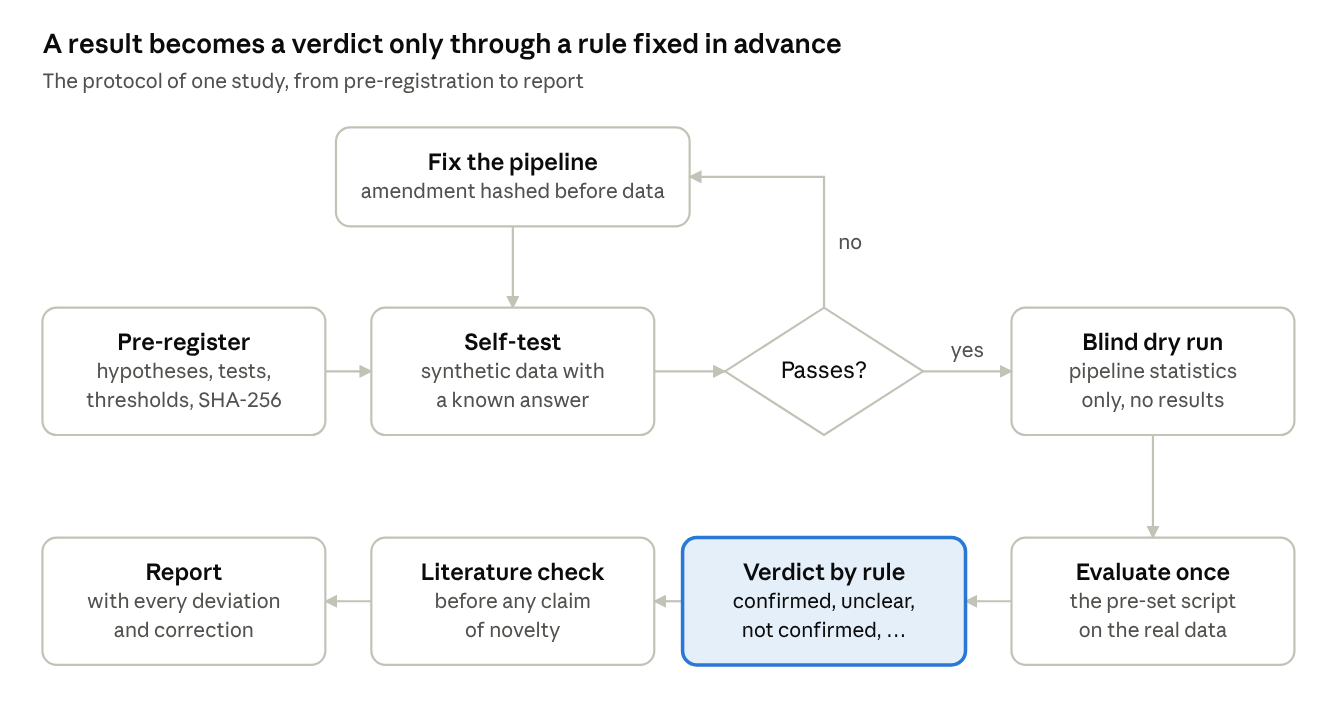
\includegraphics[width=\linewidth]{figures/fig_protocol.png}\end{center}

A failed self-test loops back to an amendment that is hashed before any real data; a change after the data is reported as a deviation (Appendix).

\textbf{Pre-registration.} Each study has a file stating the hypotheses, the primary test, the thresholds for each verdict, the budget and the stop rule. Its SHA-256 hash was recorded before any result was seen. Amendments made before the data were allowed and hashed separately; changes made after a run are labelled deviations and reported with the result.

\textbf{Self-tests.} Before touching real data, most pipelines ran on synthetic data or unchanged files whose truth was known: artificial libraries with a known attachment kernel, planted and decoy pairs for blind judges, and the unchanged mathlib files, which every Lean pipeline had to accept before a run. Self-tests caught our own errors, one of them only after it had been reported (Section 13).

\textbf{Blind dry runs.} Technical test runs on real data displayed only pipeline statistics, such as parser coverage, never the quantity being tested.

\textbf{Contamination control.} Experiments with language models used theorems added to mathlib after the models\textquotesingle{} training data; where a fixed cut date made that impossible, a clean subset was analysed separately. During runs of Claude agents, data from after the cut date were encrypted with a key outside the agents\textquotesingle{} reach; only logs of earlier agents could not be encrypted. For pull requests we used the earliest author date on the branch as the true start date.

\textbf{Verdicts.} Each confirmatory result is reported with the verdict its rule assigns:

\begin{itemize}
\tightlist
\item
  \textbf{confirmed} or \textbf{not confirmed}; \textbf{opposite} when the effect points the other way;
\item
  \textbf{unclear} when the result falls between the thresholds for the two;
\item
  \textbf{not testable} when a pre-registered precondition failed;
\item
  \textbf{no success} for a pilot that missed its goal within budget, and \textbf{stop} for a problem check that judged a problem out of reach;
\item
  \textbf{pending} for a study that is prepared, running or finished but not yet evaluated.
\end{itemize}

Anything not pre-registered is labelled exploratory or post hoc.

\textbf{Setup.}

\begin{itemize}
\tightlist
\item
  \textbf{Machines:} a laptop (Apple M4, 16 GB) for mathlib builds and the local prover models; a cloud container (2 cores, 7 GB) for Lean without mathlib, analysis and search; a small virtual machine (4 cores, 3.9 GB) for parallel jobs.
\item
  \textbf{Models under test:} DeepSeek-Prover-V2-7B and Goedel-Prover-V2-8B, both 4-bit via MLX; Claude for whole proofs, for lemma prediction and, as sub-agents, for blind judging. From 12 October also Claude Opus 5.5, Sonnet 5.5 and Haiku 4.5 through the API, GPT-6 Astra through Codex, Leanstral 1.5 through Mistral\textquotesingle s API, BFS-Prover-V2-7B locally.
\item
  \textbf{Formal states:} mathlib 1c58764af (1 September 2025) and d0a050ad6 (September 2026, Lean v4.35.0-rc2); the openai/math release pins mathlib d13f23b; the fresh theorems of Sections 5, 9 and 10 come from mathlib a02a63c2.
\item
  \textbf{Statistics:} permutation, sign, Fisher and exact McNemar tests, Wilson intervals, bootstrap over files or games, Mantel--Haenszel ratios with hypergeometric z-values. One-sided tests are used where the pre-registration fixed a direction.
\end{itemize}

\textbf{Budgets.} Pilots had explicit token and time limits. A long-proof agent cost 200,000 to 500,000 tokens; the lemma-prediction pilot cost about 5.5 million tokens. The Claude API studies of Section 9 cost roughly \$180 in total; Astra ran within a ChatGPT Pro quota, and Leanstral was free.

\section{How formal mathematics grows}

Formal libraries grow by linear preferential attachment and are maintained like good software: refactoring removes dependencies between areas about twice as often as dependencies within an area. This section condenses a separate paper draft, \emph{Wie formale Mathematik wächst} (rev 21), and adds what maintainers change inside proofs.

\textbf{Data.} Exact dependencies extracted by Lean for mathlib (269,387 → 334,777 declarations, 2025-09 → 2026-09), 71 states of Metamath\textquotesingle s set.mm (1998--2026), half-yearly states of the Archive of Formal Proofs (AFP, 2006--2026), and yearly import graphs of SymPy, Django, scikit-learn and matplotlib. An "area" is a module path to depth 3, a section of set.mm, an AFP entry or a subpackage.

\textbf{Attachment is linear.} A lemma gains new users in proportion to its current users. The exponent of the attachment kernel, fitted on lemmas with at least 10 users, is 1.005 in mathlib and 1.021 in Metamath; the AFP gives 1.004 from one user on. A common estimator, a Poisson regression on log(1 + k) over all nodes, fakes sublinear growth. Our own earlier estimate of 0.77 was this artefact; a self-test exposed it and we withdrew it.

\textbf{Refactoring removes cross-area dependencies.} Controlling for area size and target popularity, edges between areas disappear more often than edges within an area. The pre-registered tests confirmed this in all three libraries. The same test on the four Python projects gave the pre-registered verdict \emph{general}: the pattern belongs to maintained modular systems, not to mathematics.

\begin{center}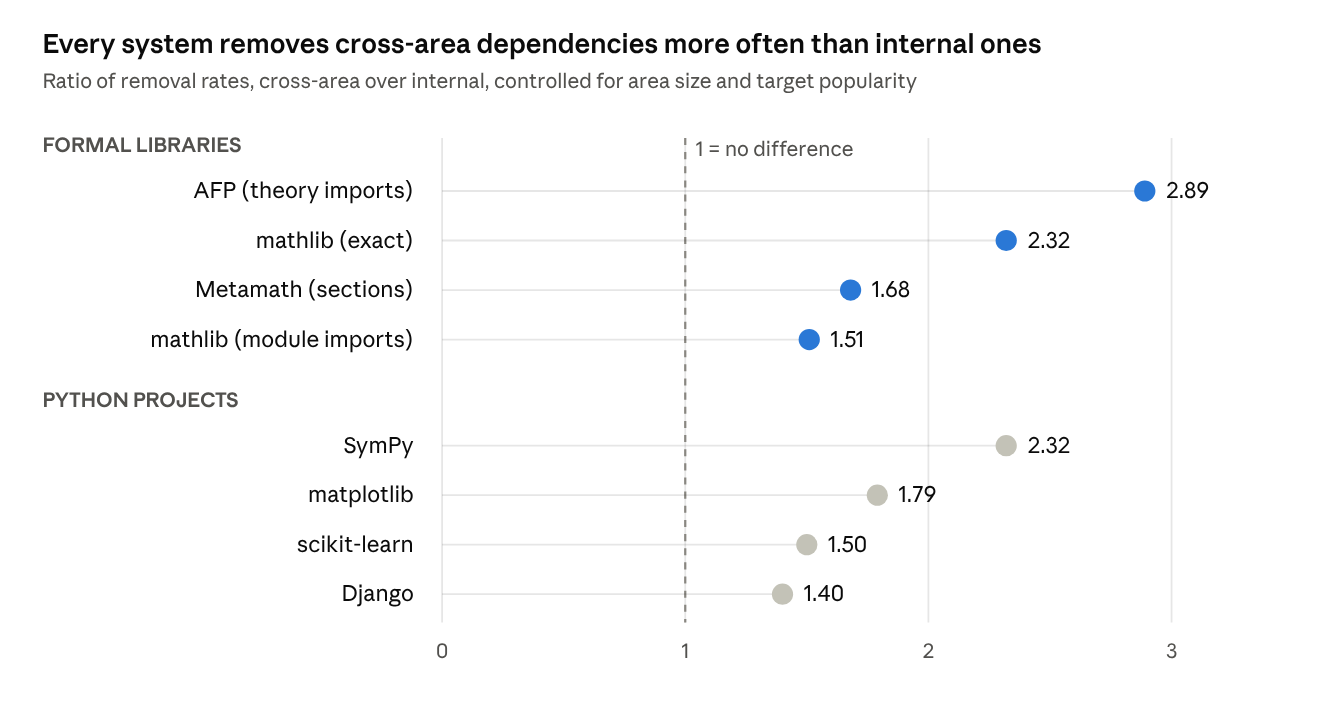
\includegraphics[width=\linewidth]{figures/fig_growth.png}\end{center}

Formal libraries and software overlap: the median of the four Python projects, 1.64, lies between mathlib\textquotesingle s module imports (1.51) and Metamath (1.68).

\begin{itemize}
\tightlist
\item
  \textbf{Scale:} in one year 834,400 of 5.62 million live mathlib edges disappeared, about 15 \%.
\item
  \textbf{Renaming does not explain it:} without targets that were deprecated, the ratio stays at 2.35 (pre-registered, \emph{robust}).
\item
  \textbf{Bundling does not explain it:} cross edges are replaced by a detour through a local lemma less often than internal ones, ratio 0.82 (pre-registered, \emph{opposite}).
\item
  \textbf{Mechanism:} In a pre-registered blind sample, read by Claude sub-agents, 113 of 120 removed cross edges point to constants Lean inserts itself, such as instances and projections. Post hoc, the ratio is 2.50 for definitions, instances and structures but only 1.17 for lemmas. In 79 \% of cases the source stays connected to the other area, so connections are rerouted rather than cut.
\item
  \textbf{Redundancy and curvature (post hoc):} over 14 monthly import graphs (304,968 edge-months, 4,787 removals), a transitively redundant import is removed with odds 1.84 {[}1.72; 1.97{]} times higher, an import between areas 1.33 {[}1.25; 1.41{]}. Jost--Liu curvature adds only 1.10 {[}1.05; 1.15{]} per standard deviation, the opposite direction to what a Ricci-flow picture suggests.
\item
  \textbf{No equilibrium:} in Metamath the share of crossing edges still rises (sections: 0.78 in 1998, 0.91 in 2026), because new cross edges arise faster than refactoring removes them.
\end{itemize}

\textbf{What maintainers change in proofs (descriptive).} Between the two mathlib states, 131,847 theorems kept their statement and 19,806 of them got a new proof. Of the 9,215 revisions that changed the sequence of tactics, 3,467 were mechanical migrations (such as \texttt{omega} → \texttt{lia}), leaving 6,015 genuine revisions. They make proofs shorter (437.8 → 380.5 characters), use fewer tactics (9.43 → 8.10), fewer named lemmas (7.26 → 5.83) and fewer \texttt{have} steps, and more automation. Where maintainers swap one named lemma for another, the new one is named explicitly less often and is more specific (mean Δlog of explicit uses −0.62), the opposite of what AI provers do (Section 4); by total use the two do not differ.

A pre-registered follow-up asked whether a model of \emph{which} proofs get revised can tell \emph{which version} maintainers keep. It cannot: on 665 deliberate revisions of similar length (within ±10 \%) it picks the new version 47.6 \% {[}43.9; 51.3{]} of the time, while "shorter is better" reaches 75.0 \%. Even within ±2 \% the new version is the shorter one in 73--84 \% of pairs.

\textbf{How predictable is growth?} Two pre-registered tests asked whether the next lemmas of mathlib can be foreseen.

\begin{itemize}
\tightlist
\item
  \textbf{From names:} a method built on mathlib\textquotesingle s naming structure hits 6.7 times as often as popularity alone (z = 11.6), so V1 was \emph{confirmed}. Yet only about 1 \% of its top 1,000 suggestions come true, far below the 10 \% set for a useful tool. What it predicts is API glue, not new mathematics.
\item
  \textbf{From file content:} Claude agents saw 20 mathlib files as of 1 June 2026 and each made 30 ranked predictions; two blind judges compared them with the 127 lemmas actually added by 21 September. The hit rate was 28 of 127, 22.0 \% {[}15.7; 30.0{]}, just under the 25 \% threshold, so the verdict is \emph{unclear}. The judges were valid (20 of 20 planted copies recognised, 0 of 9 decoys accepted, shuffled pairs 0 \%). On the 57 additions whose pull request started after 1 July the rate was 24.6 \%, so the checks showed no sign of contamination, though they cannot rule it out. Lemmanaid reports 28--50 \% for Isabelle in a comparable setting.
\end{itemize}

\section{How AI provers choose lemmas}

Where a human proof uses a rare, specific lemma, open provers reach for a popular one, and the substitute almost never works. The main cause appears to be missing knowledge rather than taste: the provers rarely use lemmas newer than their training data, though a small popularity prior exists as well (Section 5).

\textbf{The lemma-gap experiment (pre-registered).} We took 1,000 proofs of theorems added to mathlib after 1 August 2026 and removed one explicitly named lemma from each. The prover continued the proof text greedily for 32 tokens, and its first identifier was compared with the human\textquotesingle s lemma. Popularity is the number of explicit uses in LeanDojo v2 (May 2025), the period of the models\textquotesingle{} training data. The test statistic is D = log(1 + uses of the model\textquotesingle s lemma) − log(1 + uses of the human\textquotesingle s lemma).

\begin{longtable}[]{@{}
  >{\raggedright\arraybackslash}p{(\columnwidth - 4\tabcolsep) * \real{0.4333}}
  >{\raggedright\arraybackslash}p{(\columnwidth - 4\tabcolsep) * \real{0.2833}}
  >{\raggedright\arraybackslash}p{(\columnwidth - 4\tabcolsep) * \real{0.2833}}@{}}
\toprule\noalign{}
\begin{minipage}[b]{\linewidth}\raggedright
\end{minipage} & \begin{minipage}[b]{\linewidth}\raggedright
DeepSeek-Prover-V2-7B
\end{minipage} & \begin{minipage}[b]{\linewidth}\raggedright
Goedel-Prover-V2-8B
\end{minipage} \\
\midrule\noalign{}
\endhead
\bottomrule\noalign{}
\endlastfoot
same lemma as the human & 119 & 45 \\
another existing lemma & 305 & 256 \\
no lemma (a tactic, a hypothesis) & 311 & 497 \\
invented name & 211 & 153 \\
dot notation & 54 & 49 \\
mean D over lemma choices {[}95 \% CI{]} & +1.16 {[}0.93; 1.39{]} & +1.52 {[}1.20; 1.84{]} \\
popularity factor exp(D) & 3.2 & 4.6 \\
mean D, different lemmas only & +1.61 (factor 5.0) & +1.79 (factor 6.0) \\
\end{longtable}

Both primary hypotheses were \emph{confirmed} (permutation tests, p \textless{} 10\(^{-4}\)). Goedel\textquotesingle s run used a reconstructed evaluation script, which reproduces DeepSeek\textquotesingle s evaluation up to a few gaps (D = +1.15 instead of +1.16). The two provers come from different makers and base models, yet their effects do not differ clearly (+0.18 {[}−0.13; +0.49{]}); their training data overlap, so they are not fully independent.

\textbf{Where the effect sits (exploratory).} For DeepSeek, split by the popularity of the human\textquotesingle s lemma, D is +2.78 when that lemma has at most 3 uses, +1.35 for 4--29 uses and −0.16 above 29. DeepSeek replaces rare lemmas by algebra staples: \texttt{mul\_\allowbreak{}comm} 13 times, \texttt{mul\_\allowbreak{}assoc} 9 times, \texttt{add\_\allowbreak{}comm} 8 times. One example: the human\textquotesingle s \texttt{AffineSubspace.ext\_\allowbreak{}of\_\allowbreak{}direction\_\allowbreak{}eq} (6 uses) became \texttt{le\_\allowbreak{}antisymm} (1,206 uses).

\textbf{The substitutes are errors (stage 2, pre-registered).} Lean checked all 305 of DeepSeek\textquotesingle s substitutes with the rest of the human proof unchanged. Only 15 (4.9 \%) went through, 13 of them in \texttt{simp} hint lists where the hint was not needed at all. Where the human\textquotesingle s lemma was needed, the substitute worked in 0 of 114 hint lists and in 2 of 176 rewrite lists and terms, both near-synonyms. A library that checks every proof would therefore not drift towards popular lemmas; the bottleneck is finding the specific lemma.

\textbf{The knowledge-cutoff edge (pre-registered amendment).} Dating each lemma by the first of six mathlib snapshots that contains it:

\begin{itemize}
\tightlist
\item
  Goedel chose a lemma introduced after May 2025 in 2.7 \% of gaps, the human in 7.1 \% (10 gaps where only the human\textquotesingle s lemma was new, 2 where only the model\textquotesingle s was; one-sided sign test p = 0.019).
\item
  DeepSeek, evaluated alongside: 1.6 \% against 6.2 \% (14 to 0, p = 6 · 10\(^{-5}\)).
\item
  Dating names generated by attributes as old, a post-hoc sensitivity check, strengthens both results (p = 2 · 10\(^{-4}\) and 2 · 10\(^{-5}\)).
\end{itemize}

New lemmas are rarely used yet, so this edge explains part of the popularity bias mechanically.

\textbf{Maintainers go the other way.} When mathlib maintainers swap one lemma for another, they choose one that is named explicitly less often and is more specific (Δlog −0.62, Section 3); the provers move in the opposite direction (+1.16). Language models that suggest scientific references show a similar pull towards highly cited work (Algaba et al. 2025).

\textbf{An embedding test (pre-registered, not confirmed).} In a PPMI-SVD embedding of mathlib\textquotesingle s usage matrix (128 dimensions, 1.98 million edges), a lemma\textquotesingle s norm tracks its popularity and its direction its topic. The primary hypothesis, that the human\textquotesingle s lemma fits the context better by angle than the model\textquotesingle s, failed: 93 to 84 gaps, p = 0.55. Exploratory ranks agree with the reading that the model chooses by norm and the human by angle, and the embedding finds hidden premises of held-out theorems better than popularity (MRR 0.261 against 0.156).

\textbf{OpenAI\textquotesingle s and Claude\textquotesingle s proofs.} The same gap construction on 500 gaps from OpenAI\textquotesingle s formal proofs and 500 from new mathlib theorems gave DeepSeek 25.4 \% exact hits against 10.4 \% (Fisher p = 3 · 10\(^{-10}\)). The corpus effect survives control for popularity (logit 0.97, SE 0.18; pre-registered, \emph{confirmed}) and holds in every popularity tercile. Goedel replicates it: 19.2 \% against 6.8 \% (p = 2.7 · 10\(^{-9}\)). OpenAI\textquotesingle s proofs more often name the sought lemma earlier in the same proof (16 \% against 6 \%); controlling for this post hoc lowers the effect to 0.69 (SE 0.22) but does not remove it. In 116 pairs where Claude and a human proved the same theorem, Claude used older and more popular lemmas (p ≈ 10\(^{-6}\)). AI-written proofs are thus more predictable at the level of single lemma choices; Section 7 tests whether that makes them detectable.

\section{A symbolic layer around the prover}

Cheap symbolic steps around the prover raise the rate of correctly filled lemma gaps from 11.8 \% to 54.1 \% on held-out gaps, and from 15.0 \% to 45.8 \% on gaps in theorems added after the prover\textquotesingle s training data. The layer takes candidates from Lean\textquotesingle s own search, model samples, text retrieval, co-citations and a random walk on the citation graph, ranks them with a popularity correction and lets Lean check the top five. The first version already extracted almost everything its candidate list contained, so every later gain came from more candidate sources, not better ranking.

\begin{center}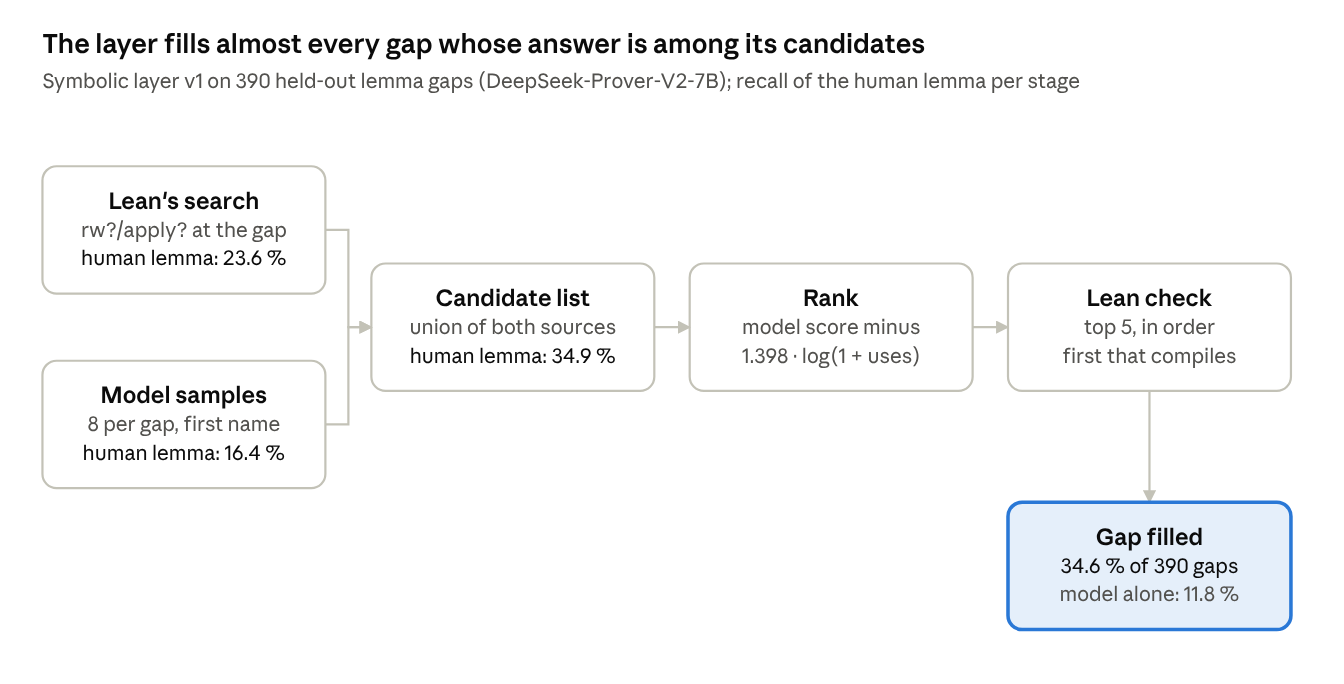
\includegraphics[width=\linewidth]{figures/fig_layer.png}\end{center}

The two sources overlap only partly, so their union raises recall from 23.6 \% to 34.9 \%; ranking and checking then turn almost all of it into filled gaps.

\textbf{Design.} All tests reuse the gaps of Section 4 whose human lemma is declared in mathlib\textquotesingle s source (800 of 1,000). Parameters were fitted on even gap numbers and tested on the odd ones (about 400 each). For the ranking tests, each gap had a candidate set of the human\textquotesingle s lemma plus up to 15 lemmas from the same file, 15 with similar names, 10 popular and 10 random ones (46 on average).

\begin{longtable}[]{@{}
  >{\raggedright\arraybackslash}p{(\columnwidth - 6\tabcolsep) * \real{0.0492}}
  >{\raggedright\arraybackslash}p{(\columnwidth - 6\tabcolsep) * \real{0.4426}}
  >{\raggedright\arraybackslash}p{(\columnwidth - 6\tabcolsep) * \real{0.3607}}
  >{\raggedright\arraybackslash}p{(\columnwidth - 6\tabcolsep) * \real{0.1475}}@{}}
\toprule\noalign{}
\begin{minipage}[b]{\linewidth}\raggedright
Test
\end{minipage} & \begin{minipage}[b]{\linewidth}\raggedright
Question
\end{minipage} & \begin{minipage}[b]{\linewidth}\raggedright
Result (DeepSeek / Goedel)
\end{minipage} & \begin{minipage}[b]{\linewidth}\raggedright
Verdict
\end{minipage} \\
\midrule\noalign{}
\endhead
\bottomrule\noalign{}
\endlastfoot
T1 & Does subtracting a popularity prior, s − α · log(1 + uses), help? & \(\hat\alpha\) = 1.40 / 0.96; top-1 0.562 → 0.582 / 0.346 → 0.382 & confirmed, small \\
T2 & Does a proximity prior (personalised PageRank) help? & \(\hat\beta\) ≈ 0, no gain & not confirmed \\
T3 & Does a "what is new" block in the context help with post-cutoff lemmas? & top-1 on lemmas newer than May 2025: 0.24 → 0.77 / 0.21 → 0.53 & confirmed, strong \\
T4a & Does the corrected ranking beat the model\textquotesingle s own top-1? & +2 to +3 points, p = 0.19 / 0.09 & not confirmed \\
T4b & How often does a Lean check of the top 5 succeed? & 84.4 \% / 70.5 \% (human lemma in the set by construction) & large, with caveat \\
N1 & Can invented names be repaired to the nearest real name? & 3.8 \% / 3.9 \% valid, threshold 5 \% & not confirmed \\
S1 & How often does Lean\textquotesingle s own search (\texttt{rw?}, \texttt{apply?}) propose the human lemma? & 23.6 \% {[}19.6; 28.0{]} of 390 gaps & "Lean\textquotesingle s search is the bottleneck" \\
S2a & Does the end-to-end layer beat free generation? (DeepSeek) & 34.6 \% against 11.8 \%; McNemar p = 2 · 10\(^{-27}\) & confirmed \\
\end{longtable}

\textbf{What the tests show.}

\begin{itemize}
\tightlist
\item
  \textbf{The prior is real but small (T1).} For Goedel the fitted α is almost exactly 1, as a Bayesian reading predicts if the model has absorbed its training prior in full. The correction mainly removes popular wrong candidates from rank 1 (37 → 14 for DeepSeek).
\item
  \textbf{Context beats reweighting for new lemmas (T3).} No reweighting can reach a lemma the model has never seen; showing it in the context can. The block contains the human lemma, so T3 measures copying, not retrieval.
\item
  \textbf{Names are not the bottleneck, types are (N1).} Repairing invented names rarely yields a valid proof step.
\item
  \textbf{Lean\textquotesingle s search and the model complement each other (S2).} Lean almost always makes suggestions (median 14), but the human lemma is among them in 23.6 \% of gaps; the model\textquotesingle s eight samples contain it in 16.4 \%, the union in 34.9 \%.
\end{itemize}

\textbf{The end-to-end layer (S2).} Candidates were Lean\textquotesingle s suggestions at the tactic containing the gap plus the first identifiers of eight model samples; the human lemma was not added. The ranking used the model\textquotesingle s score minus 1.398 · log(1 + uses). Lean checked the top five. The layer fills 20.0 \% of the 390 test gaps at rank 1 and 34.6 \% within five, against 11.8 \% for free generation. It solves 89 gaps that free generation misses and loses none. By context it fills 46.5 \% of gaps in rewrite lists, 42.3 \% in \texttt{simp} hint lists and 24.1 \% in terms. Of the filled gaps, 118 used the human lemma and 17 another one. Since 34.6 \% is close to the 34.9 \% recall of the human lemma, better ranking cannot add much; more candidate sources can.

\textbf{More candidate sources (S3--S5, pre-registered).} Each version added sources and kept the ranking and the Lean check of S2.

\begin{longtable}[]{@{}
  >{\raggedright\arraybackslash}p{(\columnwidth - 8\tabcolsep) * \real{0.0500}}
  >{\raggedright\arraybackslash}p{(\columnwidth - 8\tabcolsep) * \real{0.5333}}
  >{\raggedright\arraybackslash}p{(\columnwidth - 8\tabcolsep) * \real{0.1167}}
  >{\raggedright\arraybackslash}p{(\columnwidth - 8\tabcolsep) * \real{0.0833}}
  >{\raggedright\arraybackslash}p{(\columnwidth - 8\tabcolsep) * \real{0.2167}}@{}}
\toprule\noalign{}
\begin{minipage}[b]{\linewidth}\raggedright
Version
\end{minipage} & \begin{minipage}[b]{\linewidth}\raggedright
Sources added
\end{minipage} & \begin{minipage}[b]{\linewidth}\raggedright
pass@5 on 390 gaps
\end{minipage} & \begin{minipage}[b]{\linewidth}\raggedright
Recall of the human lemma
\end{minipage} & \begin{minipage}[b]{\linewidth}\raggedright
Test
\end{minipage} \\
\midrule\noalign{}
\endhead
\bottomrule\noalign{}
\endlastfoot
S2 & Lean\textquotesingle s \texttt{rw?}/\texttt{apply?}, eight model samples & 34.6 \% & 34.9 \% & -- \\
S3 & \texttt{exact?}, \texttt{simp?}, the 10 preceding lemmas of the same file & 39.0 \% & 42.1 \% & 21 : 4, p = 5 · 10\(^{-4}\) \\
S4 & samples from a second prover, a list of post-cutoff lemmas & 40.8 \% & 45.1 \% & 9 : 2, p = 0.03 \\
S5 & BM25 text retrieval and co-citations & 49.5 \% & 62.6 \% & 27 : 5, p = 6 · 10\(^{-5}\) \\
S5 & plus a personalised random walk (PPR) on the citation graph & \textbf{54.1 \%} & 71.5 \% & 20 : 2, p = 6 · 10\(^{-5}\) \\
\end{longtable}

All five pre-registered comparisons were confirmed (one-sided exact McNemar). The S4 gain came entirely from the second prover\textquotesingle s samples; the post-cutoff list held the human lemma at 0.5 \% of gaps. A learned graph network (LightGCN) lost to simply counting co-citations (recall at 10: 6.7 \% against 13.6 \%), while the untrained random walk was the best single source (37.4 \%).

\textbf{Is the gain an artefact? (Q1, pre-registered.)} Random theorem names fill 1.5 \% of gaps, all in \texttt{simp} hint lists where an unused hint is harmless. On the 383 gaps where the lemma is binding, S3 fills 37.9 \% and the full layer 53.3 \%, against 11.2 \% for free generation.

\textbf{Fresh gaps (N1, pre-registered).} On 400 gaps in theorems added to mathlib after the prover\textquotesingle s training data, the layer of S3 fills 41.0 \% against 15.0 \% greedy and 22.3 \% for five free samples (105 : 1 and 76 : 1, both confirmed). BM25 and co-citations add 4.3 points (27 : 10, confirmed); the random walk adds nothing here (5 : 3, not confirmed). The graph sources find the human lemma far less often on fresh gaps (PPR recall at 10: 9.5 \% against 37.4 \%), so the full layer reaches 45.8 \% instead of 54.1 \%.

\textbf{Ranking or budget? (L1, pre-registered.)} A ranking learned on the old gaps from 17 features did not beat the simple rule on the fresh ones (pass@5 46.8 \% against 45.8 \%, 19 : 15, not confirmed); its cross-validated gain was overfitting to the old gaps. Checking ten candidates instead of five is the cheap lever: 53.0 \% of fresh gaps, against 15 \% for the model alone.

\textbf{Invented names as conjectures (E1, pre-registered).} Where the prover invented a lemma name, we asked it to state what that lemma would say. Of 159 statements, 70 were well-formed, 7 fitted the gap and 5 rescued the gap with a genuine proof (confirmed at the pre-set threshold of 5, p = 0.03). The layer already fills almost all of these gaps.

\textbf{Smaller checks.} Part of the popularity prior of T1 is name length: popular lemmas have shorter names, and controlling for length lowers \(\hat\alpha\) by about 30 \% (Q2). Lemmas newer than the training data are mostly just rare: equally rare old lemmas are hit as seldom (Q3). Only 5--9 \% of invented names existed in any earlier mathlib (Q8), so a renaming table would not help.

\section{Whole proofs}

A strong model proves most new mathlib theorems, a small open prover very few, and about ten ways of helping the small prover, from lemma lists to decomposition, repair and step models, all failed. Checking needs care: a search tactic can leave a hidden \texttt{sorry} that Lean reports only as a warning. How strong models gain from Lean\textquotesingle s error messages is the subject of Section 9.

All theorems were added to mathlib after the models\textquotesingle{} training data. A proof counts only if Lean accepts it in the original file with mathlib\textquotesingle s own build options, with no error and no \texttt{sorry}.

\begin{longtable}[]{@{}
  >{\raggedright\arraybackslash}p{(\columnwidth - 6\tabcolsep) * \real{0.1833}}
  >{\raggedright\arraybackslash}p{(\columnwidth - 6\tabcolsep) * \real{0.1833}}
  >{\raggedright\arraybackslash}p{(\columnwidth - 6\tabcolsep) * \real{0.3000}}
  >{\raggedright\arraybackslash}p{(\columnwidth - 6\tabcolsep) * \real{0.3333}}@{}}
\toprule\noalign{}
\begin{minipage}[b]{\linewidth}\raggedright
Prover
\end{minipage} & \begin{minipage}[b]{\linewidth}\raggedright
Theorems
\end{minipage} & \begin{minipage}[b]{\linewidth}\raggedright
Setting
\end{minipage} & \begin{minipage}[b]{\linewidth}\raggedright
Result
\end{minipage} \\
\midrule\noalign{}
\endhead
\bottomrule\noalign{}
\endlastfoot
Claude & 57 long (25--142 human steps) & no Lean access; round 2 sees Lean\textquotesingle s errors & 41 / 57 unaided (72 \%); 42 / 57 with an outline of the human proof \\
Claude & 80 short (3--25 steps) & up to three rounds & 79 / 80 unaided; 78 / 80 with a hint on the human strategy; two repaired proofs use exact? (without them 78 and 77) \\
DeepSeek-Prover-V2-7B & 78 & 12 attempts each, 8 of them with a forced proof direction & 0 of 936 attempts \\
DeepSeek-Prover-V2-7B & 77 & given every lemma of the human proof & 2 / 77 (0 / 78 without) \\
DeepSeek-Prover-V2-7B & 160 (80 need a post-cutoff lemma) & two samples, after the recheck below & 5.0 \% and 11.3 \% \\
DeepSeek with two agents & 50 & 6 generations, as the baseline & 3 genuine, all also found by the baseline \\
\end{longtable}

\textbf{Claude.} Success falls with length (pre-registered L1, \emph{confirmed}, Cochran--Armitage p = 0.039), mainly for proofs of 50 or more human steps (3 of 9). The outline did not help (L2 undecidable, 3 to 2 discordant theorems), and the strategy hint for short proofs made no measurable difference; its hypotheses were undecidable with so few discordant pairs. The most common identified causes of failure were unknown names (20) and type or instance errors (19). No successful proof uses a search tactic, and the median similarity to the human proof is 0.15.

\textbf{How close are failed proofs? (post hoc)} Of 43 long proofs that failed in round 1 and got a fair second attempt, 25 were repaired after one round of Lean feedback. Repair succeeded for 13 of 15 proofs with one Lean error, 8 of 13 with two or three and 4 of 15 with four or more (trend p \textless{} 0.001). It also depended on where the first error sits: last third 9 of 10, middle third 9 of 12, first third 7 of 21. Error count and position may only reflect how hard a theorem is. They become a useful measure of "almost correct" only if decisions based on them (repair, restart, give up) yield more proofs than fixed rules at equal budget, which we have not tested.

\textbf{The small open prover.} DeepSeek-Prover-V2-7B fails before proof direction matters: over all attempts, 52 \% of first errors are failing tactics or type errors, 18 \% invented names and 15 \% names that exist but are unavailable at that point. Even with every lemma of the human proof and its statement in the prompt it solved only 2 of 77 theorems, so the pre-registered O1 was \emph{not confirmed}. The missing names were mostly general API, old or invented, not the few lemmas of the proof.

\begin{itemize}
\tightlist
\item
  \textbf{Drift (pre-registered):} theorems that need a lemma newer than May 2025 were not significantly harder (5.0 \% against 11.3 \%, p = 0.12), and any benefit of a list of new lemmas was not detectable at this size.
\item
  \textbf{Two agents (pre-registered, the author\textquotesingle s idea):} a fixed schedule of prover, symbolic repair, decomposition by a second agent and retries at higher temperature. Its three genuine solutions all came from the first step, the plain prover, and the baseline found the same three: P6a \emph{not confirmed}.
\item
  \textbf{Repair against restart:} repairing a failed proof with Lean\textquotesingle s error succeeded 0 of 47 times; a fresh sample succeeds about 5 \% of the time. A strong model repairs well (25 of 43 above), a 7B prover does not, though the tasks differ.
\end{itemize}

\textbf{Predicting the direction of a proof (pre-registered).} A "compass" predicts with which of eight directions a human proof starts: induction, case split, contradiction, applying a lemma, an intermediate claim, computation, rewriting or splitting the goal. From the statement alone it beats the per-area base rate (log-loss 1.631 against 1.803; 37.3 \% against 29.3 \% at rank 1) and is well calibrated (ECE 0.015); from the docstring words alone it also beats the base rate. Uncertainty about the direction did not go with longer proofs, so K3 was not confirmed. Forcing these directions on the small prover did not help (above).

\textbf{The hidden-\texttt{sorry} pitfall.} When \texttt{apply?} cannot close a goal, it admits the goal with \texttt{sorry}. Lean emits a warning, not an error, and the word \texttt{sorry} never appears in the proof text. A check that looks only for errors and for \texttt{sorry} in the text accepts such a proof. A recheck found 12 of 51 counted successes in the drift pilot and 3 of 6 agent solutions to be fake; the figures above are corrected. Claude\textquotesingle s 123 published proofs contain no search tactic (the two short-proof successes that use exact? are not among them), and the checks in Sections 4 and 5 insert resolved lemma names, so neither is affected. Any evaluation of Lean provers should treat a \texttt{sorry} warning as failure.

\textbf{Closing the small-prover line.} The runs pending on 10 October and the studies that followed all came out negative for DeepSeek-Prover-V2-7B on whole proofs:

\begin{longtable}[]{@{}
  >{\raggedright\arraybackslash}p{(\columnwidth - 6\tabcolsep) * \real{0.0508}}
  >{\raggedright\arraybackslash}p{(\columnwidth - 6\tabcolsep) * \real{0.3559}}
  >{\raggedright\arraybackslash}p{(\columnwidth - 6\tabcolsep) * \real{0.4576}}
  >{\raggedright\arraybackslash}p{(\columnwidth - 6\tabcolsep) * \real{0.1356}}@{}}
\toprule\noalign{}
\begin{minipage}[b]{\linewidth}\raggedright
Study
\end{minipage} & \begin{minipage}[b]{\linewidth}\raggedright
Idea
\end{minipage} & \begin{minipage}[b]{\linewidth}\raggedright
Result
\end{minipage} & \begin{minipage}[b]{\linewidth}\raggedright
Verdict
\end{minipage} \\
\midrule\noalign{}
\endhead
\bottomrule\noalign{}
\endlastfoot
P6b & two agents, corrected rerun & 3 / 50 against 3 / 50, the same theorems, all from the plain prover & not confirmed \\
P5 & symbolic repair of failed proofs & 11 against 9 genuine (2 : 0, p = 0.25); layer 0 of 58 & not confirmed \\
P7 & change of frame (\texttt{zify}, \texttt{push\_\allowbreak{}cast}, ...) before automation & 15 against 13 (2 : 0, p = 0.25) & not confirmed \\
HE & automation first, prover second & automation alone 0 of 160 in the theorems\textquotesingle{} own files & not confirmed \\
R2 & replace every invented name, up to four rounds & 0 of 71 genuinely repaired & not confirmed \\
D0 & likelihood as a discriminator & AUC 0.83 (own model), 0.77 (second model), beyond length & confirmed \\
D1 & rank 16 samples by likelihood & best-scored proof genuine in 10 theorems, first sample in 12 & not confirmed \\
Hull & distance to human proofs & kNN AUC 0.44, Mahalanobis 0.52: no signal & descriptive \\
UE1 & transfer the proof of a twin theorem & 37 against 35 of 160 (p = 0.25) & not confirmed \\
SF, SC & cut at the first error and fill the hole (development probes) & fills only what automation fills & not pre-registered \\
SW0 & single steps along the human proof & a step on the human path in 18.6 \% of positions & unclear \\
SW0b & the layer executes lemmas itself & net +1 at the last steps & not confirmed \\
SW0c & a step-trained model (BFS-Prover-V2-7B) & human step 8.5 \% against 18.6 \% & not confirmed \\
\end{longtable}

Three observations explain the pattern. The likelihood signal of D0 separates easy from hard theorems, not good from bad samples of one theorem (within a theorem 61 \% of pairs are ordered correctly), so it cannot pick the right sample where it matters. Retrieval answers which lemma is needed, not how to use it: human steps insert lemmas with arguments, rewrite chains and case splits, which the small model rarely writes. And invented names are invented statements: after a name is swapped, 53 of 71 proofs failed on another error. With a 7B model on a laptop, both current library knowledge and the assembly of steps are missing, and no addition we tried supplies either. The theory\textquotesingle s prediction about the spread of difficulty did hold: a beta model gave pass@16 = 12.9 \%, measured 13.1 \%, so budget should go by theorem difficulty, not by ranking samples within a theorem.

P5 was rechecked after its run with an outdated script (deviation documented); two of its four automation successes turned out spurious. P7 is reported from its third run. Q6 had suggested that automation and prover complement each other; that came from an environment containing all of mathlib, where three of the theorems are themselves \texttt{simp} lemmas, and was withdrawn after HE.

\textbf{Where proofs use their hypotheses (descriptive).} Deleting each named hypothesis of 461 new theorems (755 Lean checks) breaks the proof in almost every case. In 89.4 \% the proof names the hypothesis; in 10.6 \% automation such as \texttt{grind}, \texttt{assumption} or \texttt{simp\ {[}*{]}} consumes it silently. The first break lies at a median of one third of the proof.

\section{Detecting and auditing AI-written proofs}

AI-written Lean proofs are hard to pick out of a corpus, because the difference between application code and library code swamps the AI signal. On the same theorem, however, the AI proof is the more predictable one in 84 \% of pairs. Audits found no trivial statements in a large AI release and a proof-quality benchmark that counting lines solves.

\begin{longtable}[]{@{}
  >{\raggedright\arraybackslash}p{(\columnwidth - 6\tabcolsep) * \real{0.1967}}
  >{\raggedright\arraybackslash}p{(\columnwidth - 6\tabcolsep) * \real{0.2787}}
  >{\raggedright\arraybackslash}p{(\columnwidth - 6\tabcolsep) * \real{0.3607}}
  >{\raggedright\arraybackslash}p{(\columnwidth - 6\tabcolsep) * \real{0.1639}}@{}}
\toprule\noalign{}
\begin{minipage}[b]{\linewidth}\raggedright
Test
\end{minipage} & \begin{minipage}[b]{\linewidth}\raggedright
Data
\end{minipage} & \begin{minipage}[b]{\linewidth}\raggedright
Result
\end{minipage} & \begin{minipage}[b]{\linewidth}\raggedright
Verdict
\end{minipage} \\
\midrule\noalign{}
\endhead
\bottomrule\noalign{}
\endlastfoot
Lemma age and popularity as detector & trained on OpenAI files against new mathlib files & AUC 0.84 in training; pooled AUC 0.50 {[}0.46; 0.55{]} on 146 AI-disclosed against 714 other commits of the same projects & confirmatory tests not testable; post-hoc test fails \\
Likelihood under a prover (O2) & the same commits & AUC 0.607 (DeepSeek), 0.604 (Goedel); 0.54--0.57 within the largest project & confirmed, narrowly \\
Paired likelihood (O4) & 123 theorems proved by Claude and by a human; 2 identical proofs excluded & Claude\textquotesingle s proof more predictable in 102 / 121 (DeepSeek) and 101 / 121 (Goedel) & confirmed \\
Trivial or vacuous statements (O1) & 512 challenge declarations of openai/math & 0 closed by automation alone, 0 by deriving \texttt{False} from the hypotheses & no trivial statements found \\
Maintainer model on ProofJudge & 218 test pairs of initial and merged mathlib proofs & 84.9 \% agreement; "shorter text" 97.9 \%; "fewer lines" 100 \% & benchmark solved by length \\
\end{longtable}

\textbf{A genre confound.} The detector separated OpenAI\textquotesingle s files from new mathlib files well, but human research projects outside mathlib look like the OpenAI files. At the threshold that catches 90 \% of the training AI files, the frozen model flags 76 \% of human files in the FLT project, 45 \% in brownian-motion and 70 \% in carleson. The pre-registered confirmatory tests could not be run: the planned AI control project failed two pre-set rules (it pins an old mathlib and has only five files), and we reported this rather than changing the rules. The popularity fingerprint of 3.9 between OpenAI\textquotesingle s proofs and mathlib therefore mixes AI with genre. Comparisons with genre-matched baselines, or on the same theorem, are needed.

\textbf{Paired detection works.} Scored by mean negative log-likelihood per token under the two open provers, Claude\textquotesingle s proof beats the human proof of the same theorem in 102 and 101 of the 121 non-identical pairs (84 \% and 83 \%) (median 0.830 against 1.102 nats per token under DeepSeek; sign tests p = 3 · 10\(^{-15}\) and 2 · 10\(^{-14}\)). Without pairing, likelihood separates AI-disclosed commits only weakly, and within the largest project barely.

\textbf{Proofs as trees (exploratory).} Unfolding each file\textquotesingle s cited lemmas through mathlib\textquotesingle s citation graph (195,000 theorems), the number of reached lemmas grows slowly with depth: median mass dimension 0.8--1.2, against 1.57 for random seed sets of equal size. This holds for humans and AI alike; the prediction that AI trees are thinner failed. A combined null model, added after the single ones had been seen, attributes about 90 \% of the reduced dimension to locality (few source files) and to lemmas with few explicit dependencies.

\textbf{Audit of openai/math (7 October 2026).} The release of 6 October formalises the main results of 162 of 722 manuscripts. No challenge statement fell to standard automation or turned out vacuous, with controls that do catch easy and contradictory statements. In a fidelity audit of 30 randomly drawn main results, AI reviewers with a fixed rubric rated 7 statements as weaker than the headline claim; we spot-checked those by hand, and items rated with medium confidence still need human review.

\textbf{ProofJudge, a benchmark artefact.} ProofJudge (Caldwell 2026) evaluates LLM judges on pairs of the first and the merged version of proofs from mathlib pull requests; a good judge prefers the merged one. A maintainer model fitted only on mathlib\textquotesingle s own revision history agreed in 84.9 \% {[}79.8; 89.4{]} of 218 test pairs, above the 63.5--80.8 \% reported for six LLM judges. Yet in all 218 test pairs the merged version has fewer lines (median −37 \%), so "pick the shorter" scores 100 \%. The benchmark cannot separate a judge\textquotesingle s sense of quality from a preference for brevity.

\textbf{Pending.} A pilot on whether unused Lean material predicts what OpenAI\textquotesingle s reasoning summaries describe as abandoned approaches was pre-registered but not run.

\section{Machine-checked bounds for Rubik\textquotesingle s cube and the supercube}

In Lean 4 we proved that God\textquotesingle s number of Rubik\textquotesingle s cube lies between 20 and 28, with both directions machine-checked, together with the exact God\textquotesingle s numbers of the 2×2×2 cube and of the square group, and a lower bound of 22 for the supercube, whose face centres are oriented. The cube values are classical; as far as we found, these are the first machine-checked bounds for the 3×3×3 cube, and we found no published bound for the supercube.

\begin{longtable}[]{@{}
  >{\raggedright\arraybackslash}p{(\columnwidth - 4\tabcolsep) * \real{0.2295}}
  >{\raggedright\arraybackslash}p{(\columnwidth - 4\tabcolsep) * \real{0.3770}}
  >{\raggedright\arraybackslash}p{(\columnwidth - 4\tabcolsep) * \real{0.3934}}@{}}
\toprule\noalign{}
\begin{minipage}[b]{\linewidth}\raggedright
Lean theorem
\end{minipage} & \begin{minipage}[b]{\linewidth}\raggedright
Statement
\end{minipage} & \begin{minipage}[b]{\linewidth}\raggedright
Built from
\end{minipage} \\
\midrule\noalign{}
\endhead
\bottomrule\noalign{}
\endlastfoot
\texttt{thistlethwaite\_\allowbreak{}45} & every position is solvable in ≤ 45 face turns & Thistlethwaite\textquotesingle s four phases, 7 + 10 + 13 + 15 \\
\texttt{upper\_\allowbreak{}bound\_\allowbreak{}40} & ≤ 40 & Kociemba\textquotesingle s phase 1 (≤ 12, a certificate over 2,217,093,120 cells), then Thistlethwaite\textquotesingle s phases 3 and 4 \\
\texttt{upper\_\allowbreak{}bound\_\allowbreak{}30} & ≤ 30 & Kociemba\textquotesingle s phase 1 (≤ 12) and phase 2 (≤ 18 moves of ⟨U, D, R2, L2, F2, B2⟩) \\
\texttt{upper\_\allowbreak{}bound\_\allowbreak{}28} & ≤ 28 & pairs of phase-1 solutions whose difference avoids the 30,048 bad elements of phase 2 \\
\texttt{superflip\_\allowbreak{}distance}, \texttt{gods\_\allowbreak{}number\_\allowbreak{}bounds} & the superflip needs exactly 20 moves; hence 20 ≤ God\textquotesingle s number ≤ 28 & Reid\textquotesingle s normal form and a certified search \\
\texttt{supercube\_\allowbreak{}superflip} & the superflip with all centres unturned needs ≥ 22 moves on the supercube & the same normal form with centre signatures, symmetry reductions proved in Lean \\
\texttt{kociemba\_\allowbreak{}phase2\_\allowbreak{}lower}, \texttt{kociemba\_\allowbreak{}phase2\_\allowbreak{}attained} & the phase-2 maximum is exactly 18 & a Lipschitz certificate over 2.68 · 10\(^{9}\) cells and a witness \\
\texttt{order11\_\allowbreak{}lower}, \texttt{order11\_\allowbreak{}witness} & elements of order 11 need ≥ 10 moves; an explicit 10-move word has order 11 & a certified search \\
\texttt{slice\_\allowbreak{}group\_\allowbreak{}quarter}, \texttt{slice\_\allowbreak{}group\_\allowbreak{}half} and the anti-slice versions & God\textquotesingle s numbers 6 / 5 (slice group) and 9 / 8 (anti-slice group) & all 768 and 6,144 elements \\
\texttt{pocket\_\allowbreak{}cube\_\allowbreak{}htm}, \texttt{pocket\_\allowbreak{}cube\_\allowbreak{}qtm} & God\textquotesingle s number of the 2×2×2 is 11 in the half-turn and 14 in the quarter-turn metric & all 3,674,160 positions \\
\texttt{square\_\allowbreak{}group\_\allowbreak{}gods\_\allowbreak{}number} & God\textquotesingle s number of ⟨U2, R2, F2, D2, L2, B2⟩ is 15 & all 663,552 elements \\
\texttt{parity\_\allowbreak{}law} & corner and edge permutation parities agree & a pure proof \\
\end{longtable}

\textbf{The phase bounds are tight.} For each phase, the distance table was checked to be 1-Lipschitz along the phase\textquotesingle s moves, and an explicit witness attains the maximum. So 45 and 40 are the best these decompositions can give. The bound 30 = 12 + 18 is the plain two-phase bound; Reid (1995) sharpened it to 29, and the true value is 20 (Rokicki et al. 2013).

\textbf{Certifying phase 2.} In phase 2 every piece is oriented, so a position is a pair of a corner and an edge permutation: 19.5 · 10\(^{9}\) group elements. The 16 symmetries that fix the U--D axis cut the corner permutations to 2,768 classes. For the 444 classes with a nontrivial stabiliser the edge index had to be canonicalised; without that, the first descent check failed. This left 2,678,538,240 cells of one byte each. A compiled breadth-first search filled the table, and a check confirmed for every reachable cell (even parity, canonical form) that its distance is at most 18, is 0 only at the solved cell, and otherwise drops by one along some move. The certificate took about 87 minutes and 3.6 GB.

\textbf{Trust base and validation.} The proofs use Lean 4.23.0 core without Mathlib. Besides the three standard axioms they rely on \texttt{native\_\allowbreak{}decide}, so the tables are checked by compiled code rather than by the kernel; \texttt{parity\_\allowbreak{}law} uses no \texttt{native\_\allowbreak{}decide}. Three external checks tie the formal model to the physical cube:

\begin{itemize}
\tightlist
\item
  the phase-1 distance distribution equals the one Michael Reid published in 1995, cell count for cell count;
\item
  the 2×2×2 distance distributions equal the published ones;
\item
  a solver built only from the certified tables solved 50 real competition scrambles in 21--33 moves (mean 28.1), each confirmed by an independent sticker simulator.
\end{itemize}

\textbf{Novelty.} Théry (2008) verified the 2×2×2 cube in Coq, and a Lean library (vihdzp/Rubik) proves the solvability criterion and the group order without bounds. We found no earlier machine-checked upper bound for the 3×3×3 cube; the AFP, Rocq libraries and the Lean Zulip have not yet been searched. A separate paper draft describes this work in detail.

\textbf{Why two phases cost less than the sum of their maxima (exploratory).} Cutting any optimal solution after its last move outside the phase-2 group H gives an exact formula: the distance of g is the minimum, over all phase-1 solutions w, of \textbar w\textbar{} plus the phase-2 distance of g·w. The sum 12 + 18 bounds only the shortest phase-1 solution; minimising over all of them brings the value down to 20.

\begin{itemize}
\tightlist
\item
  \textbf{A check:} the superflip has exactly 792,256 phase-1 solutions of length 12, the number Dik Winter reported in 1992.
\item
  \textbf{Typical positions:} the endpoints of phase-1 solutions behave almost like independent random elements of H. Each extra phase-1 move gives 17--20 times more choices, and each lowers the best reachable phase-2 length by 1.7--1.9 moves.
\item
  \textbf{Symmetric positions:} the superflip\textquotesingle s solutions collapse about 20-fold under symmetry, and the remaining ones are correlated, which is why symmetric positions are extreme.
\item
  \textbf{A model of God\textquotesingle s number:} with the independence measured at short lengths, the model predicts the maximum of 20 correctly but is far too optimistic in the bulk. A level of independence that fits the bulk predicts 22. No single level fits both; the growing correlation between long phase-1 solutions is the part without a known structural description.
\end{itemize}

\textbf{From 30 to 28 (proved 10 October).} Two phase-1 solutions w, w′ of the same coset differ by one element k of the phase-2 group H, the same k for every position of the coset. A position needs more than 28 moves only if all its alternatives are bad at once. Only 30,048 elements of H can lead from one distance-18 element to another, out of 1.95 · 10\(^{10}\). Cosets at phase-1 distance at most 10 give 10 + 18 directly; for each of the 58,202,444 cells at distance 11 one suitable pair of words sufficed, and for the 476 cells at distance 12 three to twelve words per cell move every element of distance 17 or more below 17. The certificates took about 2.5 hours. The bound is Radu\textquotesingle s 28 from 2005; what is new is only the formal check.

\textbf{The lower bound 20 (proved 10 October).} The superflip is central in the cube group, so cyclic shifts, symmetry images and inverses of a solution are again solutions. Reid\textquotesingle s 1995 normal form uses this to cut the search; we certified it in Lean with the phase tables of the upper bounds, about 1.7 · 10\(^{8}\) search nodes. With the explicit 20-move solution this proves \texttt{gods\_\allowbreak{}number\_\allowbreak{}bounds}. As far as we know this is the first machine-checked lower bound on the 3×3×3 God\textquotesingle s number; the mathematics is Reid\textquotesingle s.

\textbf{The supercube (proved 11 October).} If the face centres carry an orientation, a position is a cube element plus a centre pattern. Counting move sequences gives only ≥ 21. The central elements are the superflip times any of 2,048 even centre patterns. A search over all superflip words of length ≤ 21 in normal form, with their centre signatures, reached only 624 patterns, so every other pattern needs ≥ 22 moves: the plain superflip, the superflip with all centres turned by 180°, and 1,422 more. Two pre-registered predictions held (at most five symmetry orbits reached at length 20: 2; fewer than half the patterns by length 21: 624). For the unturned centres the bound is proved in Lean (\texttt{supercube\_\allowbreak{}superflip}, about 9 hours of certified search); together with a sticker-verified 254-move witness this gives a supercube God\textquotesingle s number of at least 22. We found no published bound.

\textbf{A clumping law for hard positions (pre-registered).} If the solutions of a position come in orbits of size s under its symmetries, and orbits behave like independent darts, then P(distance \textgreater{} k \textbar{} s) ≈ P(distance \textgreater{} k)\^{}(1/s). On all 164.6 billion symmetric positions counted by Rokicki, the share at distance 20 follows this law over five orders of magnitude with no free parameter (slope −0.71 ± 0.07 against a predicted −1; the five order-2 classes within a factor 3.2 of the prediction), so the hypothesis was supported, but only for the extreme tail: at distance ≥ 19 and on the 2×2×2 the predicted slope failed. Exploring further, all 32 antipodes of the tipless pyraminx are central elements. We found neither the law nor the pyraminx observation in the literature.

\textbf{Puzzle groups in GAP (7 October).} As side work, sticker-group orders were computed in GAP: about 1.8 · 10\(^{44}\) for the 4×4×6 cuboid, cross-checked in Python, and about 10\(^{720}\) for the Teraminx, with a structural argument via Goursat\textquotesingle s lemma. For the Latch Cube, whose legal moves depend on the state, an exhaustive search reproduced every published count of reachable arrow configurations.

\section{Repair with Lean feedback}

For frontier models the decisive lever is a loop that hands Lean\textquotesingle s error messages back to the model. On 233 fresh mathlib theorems Claude Opus 5.5 proved 229 with one proof and up to three repairs, against 204 with four independent attempts at the same number of Lean checks, at a third of the cost. The gain needs a minimum model strength, comes mostly from the content of the messages, and was replicated with GPT-6 Astra.

All theorems entered mathlib (state a02a63c2) after the models\textquotesingle{} training data; a proof counts as in Section 6. Unless stated otherwise each theorem had at most four Lean checks. Opus ran with adaptive thinking at the default effort (in Z1 at effort low) through the API, Astra through the Codex command line, all without web access. Two settings recur: the file up to the statement, or only the file\textquotesingle s header lines and the statement ("bare"), which removes nearby lemmas from view.

\begin{longtable}[]{@{}
  >{\raggedright\arraybackslash}p{(\columnwidth - 6\tabcolsep) * \real{0.0492}}
  >{\raggedright\arraybackslash}p{(\columnwidth - 6\tabcolsep) * \real{0.3115}}
  >{\raggedright\arraybackslash}p{(\columnwidth - 6\tabcolsep) * \real{0.4590}}
  >{\raggedright\arraybackslash}p{(\columnwidth - 6\tabcolsep) * \real{0.1803}}@{}}
\toprule\noalign{}
\begin{minipage}[b]{\linewidth}\raggedright
Study
\end{minipage} & \begin{minipage}[b]{\linewidth}\raggedright
Model, theorems
\end{minipage} & \begin{minipage}[b]{\linewidth}\raggedright
Result
\end{minipage} & \begin{minipage}[b]{\linewidth}\raggedright
Verdict
\end{minipage} \\
\midrule\noalign{}
\endhead
\bottomrule\noalign{}
\endlastfoot
O1 & Opus, 397 fresh lemma gaps & pass@10 88.7 \% alone, 89.7 \% with 10 candidates of the layer (14 : 10, p = 0.27); Opus alone beats layer plus 7B prover 154 : 11 & not confirmed / confirmed \\
O2 & Opus, 233 theorems, file & repair 229, four fresh attempts 204 (26 : 1, p = 4 · 10\(^{-7}\)); \$0.076 against \$0.225 per theorem & confirmed \\
O3 & Opus, 191 theorems needing a fresh lemma, bare & repair 151, repair with the layer 177 (31 : 5, p = 6.5 · 10\(^{-6}\)); first attempt 63 against 99 & confirmed \\
O4 & Opus with its own search tool, 95 of them & 91 against 87 with the layer (5 : 1, p = 0.22); first attempt 64 against 51 (p = 0.015); search against plain repair 13 : 0 & partly confirmed \\
O5 & Haiku 4.5, Sonnet 5.5, Opus 5.5, 100 theorems & repair 21 / 98 / 100 against four attempts 16 / 84 / 89; repair rate per round 0.05 / 0.60 / 0.72 & Sonnet confirmed, Haiku no difference \\
A1 & Astra, 187 theorems, bare & repair 118 against four attempts 47 (72 : 1); with the layer 150 (37 : 5); with search in the source tree 89 of 91 (28 : 0) & all three confirmed \\
A2 & Astra at three reasoning efforts & repaired after a failed first attempt: low 55 \%, medium 56--64 \%, high 65 \% & not confirmed \\
E1 & Astra, 191 theorems, three kinds of feedback & full messages 103, line numbers only 51, "Lean rejected this proof" 50 & content matters, position alone does not \\
P1 & Astra, 57 long theorems (25--142 human steps), up to 10 calls & with search 57 of 57, without 53 of 57 (4 : 0, p = 0.06); a self-written outline repaired step by step solved fewer & not confirmed (ceiling) \\
Z1 & Opus, 99 Omni-MATH problems, a checker of form only & certified answers 85 → 97 (p = 5 · 10\(^{-4}\)), correct answers 73 → 79 (p = 0.15) & confirmed, weakly \\
PB1 & Astra, 20 random PutnamBench problems & 20 of 20 within at most 10 calls (mean 2.4), 8 at the first attempt; standard axioms only & pilot \\
G0 & Goedel-Prover-V2-8B on the laptop, 10 theorems & 0 of 10; corrections repeat the same proof & pilot, no success \\
\end{longtable}

\textbf{A threshold of model strength, not of thinking time.} The ratio of repair success to the success of a fresh attempt is similar for Haiku, Sonnet and Opus (2.1--3.3). What differs is the level: one round of repair succeeds 5 \% of the time for Haiku, 60 \% for Sonnet and 72 \% for Opus, and Sonnet with repair nearly matches Opus at half the price. Within one model, more reasoning effort helped only modestly (Astra 55 \% to 65 \% from low to high), so the threshold lies in the model, not in its thinking budget.

\textbf{What the message carries (E1).} Repair multiplies the per-round success of a fresh attempt (0.04) by about 7. About a factor 2 comes from seeing one\textquotesingle s own failed attempt (0.08 with a bare rejection), and about 3.5 from the content of the message: the missing name, the mismatched type, the open goal. Line numbers alone add nothing. Z1 shows the flip side: with a checker that tests only the form of an answer, repair raised coverage but not correctness, and 4 of 18 repaired answers were wrong.

\textbf{Errors multiply over steps (F1, pre-registered).} First-attempt success falls exponentially with the length of the human proof for all six sources (F1a confirmed), and weaker models lose more per line (F1b confirmed). The implied success per line is 0.95 for Opus, 0.93 for Sonnet, 0.82 for Astra in the bare setting, 0.75 for the 7B prover and 0.69 for Haiku. This is why repair, which only has to fix the failing steps, pays most for long proofs.

\textbf{Layer or own search?} The layer helps Opus exactly where it supplies a fresh lemma: on 112 theorems where it does, repair with the layer solved 111 against 83; on 79 where it does not, 66 against 68 (post hoc). Given a simple search tool, Opus finds what it needs itself and is at least as good, but the layer is about 45 \% cheaper per solved theorem. A pre-registered recall test (F2) explains the pattern: the layer finds the fresh, topical lemmas (0.87 per lemma at 200 candidates) but rarely the general tool lemmas a proof also needs, so over all needed lemmas it reaches only 0.41; it cannot substitute for a model that knows those.

\textbf{Contamination and saturation.} Opus\textquotesingle s proofs share little text with the human ones (median share of identical lines 0.00; at least 90 \% in 71 of 921 genuine proofs, 56 of them where a twin theorem stood in the context). Public pull requests before the cut-off cannot be ruled out. The fresh theorems are nearly saturated for Opus with its file (98 \%), so the bare setting and PutnamBench were used for harder tests.

\textbf{A methodological finding.} A coding agent with network access used web search in 27 repair rounds, partly for the theorem itself: in Codex, the setting that disables web search did not apply when a session was resumed. These rounds and every later round of the same session were counted as failures. Only the command log revealed it.

\section{An open Lean model: Leanstral}

Leanstral 1.5, Mistral\textquotesingle s open model for Lean (a mixture of experts with 119 billion parameters, about 6.5 billion active, released on 30 June 2026), solved 66 of 95 fresh theorems as an agent that could read and search the current mathlib sources. That places it between the small provers and Opus. Five pre-registered attempts to improve it failed, and forcing it into a fixed check loop without search lowered it to 31--46.

\begin{center}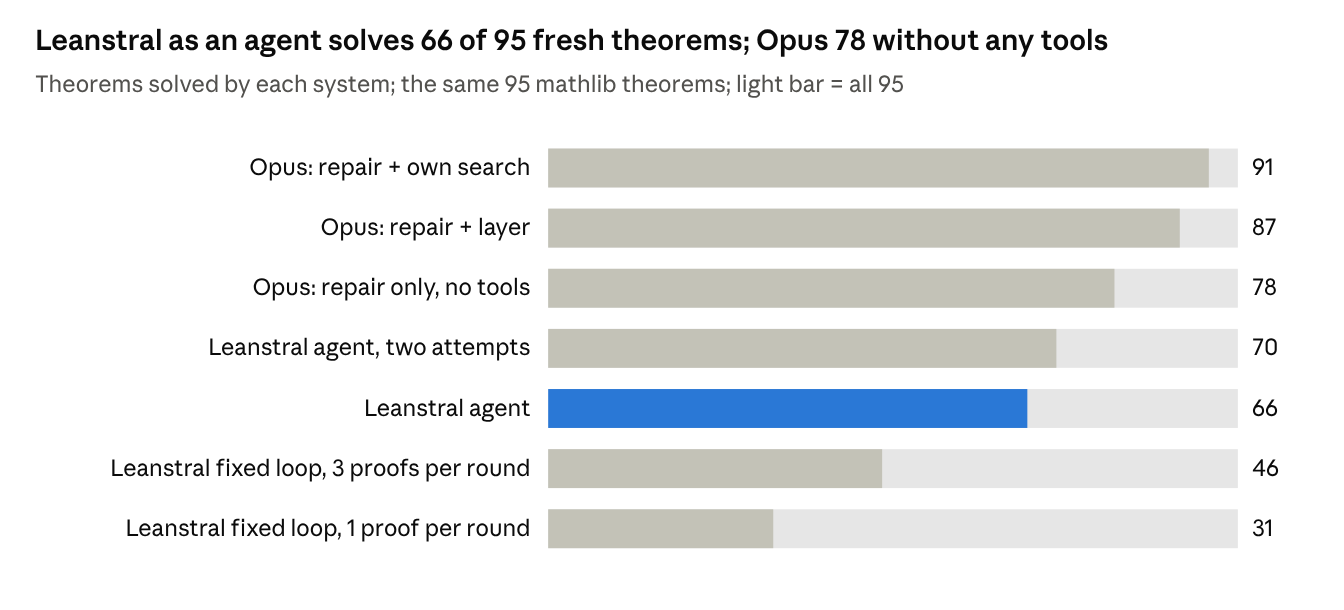
\includegraphics[width=\linewidth]{figures/fig_leanstral.png}\end{center}

The 95 theorems are those of O4, so every bar is paired. Opus saw only the header and the statement (bare setting) with at most four Lean checks; the Leanstral agent saw the file and the sources and could check as often as its time allowed, so the comparison favours Leanstral. The two-attempt bar counts a second, unchanged agent run on the 29 theorems the first one missed.

\begin{longtable}[]{@{}
  >{\raggedright\arraybackslash}p{(\columnwidth - 6\tabcolsep) * \real{0.0500}}
  >{\raggedright\arraybackslash}p{(\columnwidth - 6\tabcolsep) * \real{0.4667}}
  >{\raggedright\arraybackslash}p{(\columnwidth - 6\tabcolsep) * \real{0.3667}}
  >{\raggedright\arraybackslash}p{(\columnwidth - 6\tabcolsep) * \real{0.1167}}@{}}
\toprule\noalign{}
\begin{minipage}[b]{\linewidth}\raggedright
Study
\end{minipage} & \begin{minipage}[b]{\linewidth}\raggedright
Setting
\end{minipage} & \begin{minipage}[b]{\linewidth}\raggedright
Result
\end{minipage} & \begin{minipage}[b]{\linewidth}\raggedright
Verdict
\end{minipage} \\
\midrule\noalign{}
\endhead
\bottomrule\noalign{}
\endlastfoot
O3L & the chat loop of Opus R and RS, bare setting & 0 of 5 pilot theorems; stopped & no success \\
O3LA & agent (Mistral Vibe), 600 s and 60 turns, mathlib sources cut before each theorem, a Lean check script & 66 of 95; Opus without tools 78 (20 : 8, p = 0.036) & descriptive \\
O3LA2 & on the 29 unsolved: plain restart, a rule to commit early, a relay of three short sessions & 4, 8 and 5 of 29 & not confirmed \\
O3LA3 & goal states at every \texttt{sorry} in the check output & 53 of 95 strictly; 69 against 68 without the isolation rule & not confirmed \\
O3LA3, second arm & Lean language-server tools & the model never called them in the agent harness & dropped \\
LS1 & no agent: fixed loop of proof, Lean errors and the layer\textquotesingle s name hints; one or three proofs per round & 31 and 46 of 95; three against one proof per round 16 : 1, p = 3 · 10\(^{-4}\) & not confirmed \\
\end{longtable}

\textbf{Where it fails.} The protocols show that Leanstral finds the fresh lemmas it needs: in 11 of 13 failures where the layer would have supplied one, the agent had already found it by searching. It fails at assembling the proof. In failed attempts the errors were type mismatches (72), failing tactics (59) and open goals (55); unknown names appeared only 9 times. Unsolved runs made a median of 64 calls (mean 61), about 39 of them searching and reading, and ran Lean only 5.6 times on average; 9 of the 29 never left a proof in the file, and a rule to commit after ten searches was mostly ignored.

\textbf{Why the fixed loop is worse.} Without the ability to search, every fourth candidate in LS1 used an invented name, and the layer\textquotesingle s hints caught only part of them. Of the 22 theorems only the agent solved, 14 ended in the loop with a single remaining error, usually a detail of assembly (a rewrite that finds no pattern, a mismatched type) that the agent resolves by reading the definition or a neighbouring proof. Within the loop, more attempts per round helped clearly, as the product law predicts, but at a much lower level.

\textbf{Isolation.} Each agent ran in a sandbox whose mathlib sources were cut before the target theorem; every tool call was logged and audited. Runs that touched files outside the sandbox were counted as failures even when harmless (6 in O3LA). In O3LA3 our check script exposed the path to the full mathlib, and the agent used it in 11 runs; the strict count excludes them, and the run is reported only as an upper bound for the benefit of the extra feedback.

\section{Auditing formal-conjectures}

An AI audit of formal-conjectures, Google DeepMind\textquotesingle s collection of formalised open problems, found two statements listed as open that are false as formalised; Lean checks both disproofs with the standard axioms only.

\textbf{The audit (F2).} GPT-6 Astra, with search in the repository, judged 1,097 of the 1,244 statements marked open at commit 84cf7f8 before its quota ran out; it flagged 5 as defective, and for 2 it produced a disproof that Lean accepts.

\begin{longtable}[]{@{}
  >{\raggedright\arraybackslash}p{(\columnwidth - 4\tabcolsep) * \real{0.2333}}
  >{\raggedright\arraybackslash}p{(\columnwidth - 4\tabcolsep) * \real{0.5500}}
  >{\raggedright\arraybackslash}p{(\columnwidth - 4\tabcolsep) * \real{0.2167}}@{}}
\toprule\noalign{}
\begin{minipage}[b]{\linewidth}\raggedright
Statement
\end{minipage} & \begin{minipage}[b]{\linewidth}\raggedright
Defect
\end{minipage} & \begin{minipage}[b]{\linewidth}\raggedright
Status
\end{minipage} \\
\midrule\noalign{}
\endhead
\bottomrule\noalign{}
\endlastfoot
\texttt{rudins\_\allowbreak{}conjecture\_\allowbreak{}unique} & Claims that for every N ≥ 6 each non-trivial arithmetic progression with the maximal number of squares among its first N terms has difference 24. At N = 6, 120n + 49 has four squares (49, 169, 289, 529), as many as the maximum, with difference 120. The source (González-Jiménez and Xarles 2014) claims uniqueness only up to equivalence and only for certain N ≥ 8. & disproof checked in Lean \\
\texttt{erdos\_\allowbreak{}70}, variant \texttt{omega\_\allowbreak{}one} & Claims \(\mathfrak{c} \to (\omega_1, n)^3_2\) for all n ≥ 2. Colour a triple blue when its middle element is a peak under a bijection with the reals: no four elements are all blue, and every red set is countable, so the claim fails for n = 4 in ZFC. The result is in Erdős, Hajnal and Rado (1965, Theorem 11), so the variant is known and mislabelled as open. & disproof checked in Lean; literature found afterwards \\
\end{longtable}

The main problem of Erdős \#70 is not affected. A report to the maintainers is in preparation. Three further flags (two on \texttt{erdos\_\allowbreak{}897} variants, one on an Erdős \#887 variant) have no Lean proof and do not count.

\section{Overview of all verdicts}

The tables list the pre-registered decisions of the studies in this edition with their verdicts. Hashes are the first eight hex digits of each file\textquotesingle s SHA-256.

\subsection*{Formal mathematics and AI provers (Sections 3--7)}
\addcontentsline{toc}{subsection}{Formal mathematics and AI provers (Sections 3--7)}

\begin{longtable}[]{@{}
  >{\raggedright\arraybackslash}p{(\columnwidth - 8\tabcolsep) * \real{0.2787}}
  >{\raggedright\arraybackslash}p{(\columnwidth - 8\tabcolsep) * \real{0.0492}}
  >{\raggedright\arraybackslash}p{(\columnwidth - 8\tabcolsep) * \real{0.2131}}
  >{\raggedright\arraybackslash}p{(\columnwidth - 8\tabcolsep) * \real{0.3443}}
  >{\raggedright\arraybackslash}p{(\columnwidth - 8\tabcolsep) * \real{0.1148}}@{}}
\toprule\noalign{}
\begin{minipage}[b]{\linewidth}\raggedright
Study
\end{minipage} & \begin{minipage}[b]{\linewidth}\raggedright
§
\end{minipage} & \begin{minipage}[b]{\linewidth}\raggedright
Pre-registration
\end{minipage} & \begin{minipage}[b]{\linewidth}\raggedright
Main result
\end{minipage} & \begin{minipage}[b]{\linewidth}\raggedright
Verdict
\end{minipage} \\
\midrule\noalign{}
\endhead
\bottomrule\noalign{}
\endlastfoot
Cross-area removal, Metamath & 3 & \texttt{VORAB\_\allowbreak{}METAMATH} 1bf01ba2 & ratio 1.68, z = 54 & confirmed \\
Cross-area removal, AFP & 3 & \texttt{VORAB\_\allowbreak{}AFP} 2432b0b1 & ratio 2.89, z = 10 & confirmed \\
Cross-area removal, mathlib exact & 3 & \texttt{VORAB\_\allowbreak{}EXAKT} d68ea81d & ratio 2.32, z = 206, 6 of 6 size bands & confirmed \\
Is the pattern specific to mathematics? & 3 & \texttt{VORAB\_\allowbreak{}SOFTWARE} dab81899 & no: pre-registered verdict "general" (four Python projects, median 1.64) & not confirmed \\
Robust to renaming (R) & 3 & \texttt{VORAB\_\allowbreak{}MECHANISMUS} 584f29fe & ratio stays 2.35 without deprecated targets & confirmed \\
Bundling via local lemmas (M1) & 3 & \texttt{VORAB\_\allowbreak{}MECHANISMUS} 584f29fe & ratio 0.82 & opposite \\
Next lemmas from names (V1) & 3 & \texttt{VORAB\_\allowbreak{}VORHERSAGE} 8e6726dc & 6.7 times popularity, but about 1 \% of the top 1,000 & confirmed \\
Next lemmas from file content & 3 & \texttt{VORAB\_\allowbreak{}LUECKEN} c804efc3 & 22.0 \% {[}15.7; 30.0{]}, threshold 25 \% & unclear \\
Revision model picks the kept version & 3 & \texttt{laengentest\_\allowbreak{}VORAB} 76e25f6e & 47.6 \%; "shorter" 75.0 \% & not confirmed \\
Popular substitutes, DeepSeek & 4 & \texttt{PRAEREGISTRIERUNG\_\allowbreak{}LUECKEN} cc1c5efd & D = +1.16, factor 3.2 & confirmed \\
Substitutes checked by Lean (stage 2) & 4 & the same file with stage 2 added, 38712daf & 15 of 305 type-check & descriptive \\
Popular substitutes, Goedel & 4 & \texttt{VORAB\_\allowbreak{}ZWEITMODELL} 090421e2 & D = +1.52, factor 4.6 & confirmed \\
Knowledge-cutoff edge & 4 & \texttt{VORAB\_\allowbreak{}ZWEITMODELL\_\allowbreak{}ALTER} c3a216cd & new lemmas 2.7 \% against 7.1 \%, p = 0.019 & confirmed \\
Human lemma fits context better by angle & 4 & \texttt{dualraum\_\allowbreak{}VORAB} cdb561c5 & 93 to 84 gaps, p = 0.55 & not confirmed \\
OpenAI\textquotesingle s lemmas easier to predict (O3) & 4 & \texttt{VORAB\_\allowbreak{}OLUECKEN} 89d32469 & 25.4 \% against 10.4 \%; logit 0.97 after popularity control & confirmed \\
The same with Goedel & 4 & \texttt{VORAB\_\allowbreak{}OLUECKEN\_\allowbreak{}GOEDEL} 4bd296e9 & 19.2 \% against 6.8 \% & confirmed \\
T1: popularity prior & 5 & \texttt{VORAB\_\allowbreak{}THEORIE} f78a3bb3 & top-1 +2.0 and +3.6 points & confirmed \\
T2: proximity prior & 5 & \texttt{VORAB\_\allowbreak{}THEORIE} f78a3bb3 & no gain & not confirmed \\
T3: "what is new" block & 5 & \texttt{VORAB\_\allowbreak{}THEORIE} f78a3bb3 & top-1 on new lemmas 0.24 → 0.77 and 0.21 → 0.53 & confirmed \\
T4a: corrected ranking & 5 & \texttt{VORAB\_\allowbreak{}T4} abde5684 & +2 to +3 points, not significant & not confirmed \\
T4b: Lean check of the top 5 & 5 & \texttt{VORAB\_\allowbreak{}T4} abde5684 & 84.4 \% and 70.5 \%, human lemma in the set & descriptive \\
N1: repairing invented names & 5 & \texttt{VORAB\_\allowbreak{}NAMEN} 8dcd607b & 3.8 \% and 3.9 \%, threshold 5 \% & not confirmed \\
S1: recall of Lean\textquotesingle s search & 5 & \texttt{VORAB\_\allowbreak{}SUCHE} e1ead8d0 & 23.6 \%, read as "Lean\textquotesingle s search is the bottleneck" & descriptive \\
S2a: end-to-end layer & 5 & \texttt{VORAB\_\allowbreak{}S2} 957ed452 & 34.6 \% against 11.8 \% & confirmed \\
S3: more candidate sources & 5 & \texttt{VORAB\_\allowbreak{}S3} 34782b20 & 39.0 \% against 34.6 \% (21 : 4, p = 5 · 10\(^{-4}\)) & confirmed \\
S4: Goedel and post-cutoff sources & 5 & \texttt{VORAB\_\allowbreak{}S4} f1a1e443 & 40.8 \% against 39.0 \% (9 : 2, p = 0.03) & confirmed \\
Long proofs by Claude (L1--L3) & 6 & \texttt{VORAB\_\allowbreak{}LANG} ef8dbf4f & 41 of 57; L1 confirmed, L2 undecidable, L3 not & partly confirmed \\
Strategy hint for short proofs & 6 & \texttt{VORAB\_\allowbreak{}KOMPASS\_\allowbreak{}STARK} 75b5377e & 79 of 80 without, 78 of 80 with; both hypotheses undecidable & not testable \\
Forced proof directions, DeepSeek & 6 & \texttt{richtung/\allowbreak{}VORAB\_\allowbreak{}FESTLEGUNG} 1e19d617 & 0 of 936 attempts & not testable \\
Lemma oracle, DeepSeek (O1) & 6 & \texttt{orakel/\allowbreak{}VORAB\_\allowbreak{}FESTLEGUNG} e1e5f499 & 2 of 77, at least 5 required & not confirmed \\
Bridges between areas & 6 & \texttt{brueken/\allowbreak{}VORAB} ad167429 & 0 of 71 targets closed & descriptive \\
Drift: post-cutoff theorems, lemma list (D1, D2) & 6 & \texttt{VORAB\_\allowbreak{}DRIFT} 119bb0dd & 5.0 \% against 11.3 \%, p = 0.12; list effect not detectable at this size & not confirmed \\
Two agents (P6a) & 6 & \texttt{VORAB\_\allowbreak{}P6} 18cba08b & 3 genuine solutions, all also by the baseline & not confirmed \\
Two agents, corrected rerun (P6b) & 6 & \texttt{VORAB\_\allowbreak{}P6B} f307ffe6 & 3 of 50 against 3 of 50, the same theorems & not confirmed \\
Symbolic repair of whole proofs (P5) & 6 & \texttt{VORAB\_\allowbreak{}P5} 634b6399 & 11 against 9 genuine (2 : 0, p = 0.25), after recheck & not confirmed \\
Change of frame before automation (P7) & 6 & \texttt{VORAB\_\allowbreak{}P7} 06f2c290 & 15 against 13 (2 : 0, p = 0.25) & not confirmed \\
Direction of a proof from its statement (K1--K4) & 6 & cited in \texttt{kompass/\allowbreak{}ERGEBNIS.md} & K1, K2, K4 confirmed; K3 not & partly confirmed \\
Likelihood as discriminator for generated proofs (D0) & 6 & \texttt{VORAB\_\allowbreak{}D0} f7b39a1e & AUC 0.83 and 0.77, beyond length & confirmed \\
Generated proofs inside the hull of human proofs & 6 & \texttt{VORAB\_\allowbreak{}HUELLE} ccce7085 & no signal (kNN AUC 0.44, Mahalanobis 0.52) & descriptive \\
Detection by lemma age and popularity & 7 & \texttt{VORAB\_\allowbreak{}DETEKTION} c651b0dc & control failed pre-set rules; post hoc AUC 0.50 & not testable \\
AI proof trees are thinner (E1) & 7 & \texttt{VORAB\_\allowbreak{}FRAKTAL} de584334 & exploratory: thicker in training, no held-out difference & descriptive \\
Null models for tree dimension & 7 & \texttt{VORAB\_\allowbreak{}FRAKTAL\_\allowbreak{}NULL} 25eea040 & single nulls below 0.9; a combined null added post hoc explains about 90 \% & descriptive \\
Trivial challenge statements (O1) & 7 & \texttt{VORAB\_\allowbreak{}SCAN} 951a1e27 & 0 of 512 & descriptive \\
Likelihood detects AI commits (O2) & 7 & \texttt{VORAB\_\allowbreak{}PPL} ae909924 & AUC 0.607 and 0.604 & confirmed \\
Paired likelihood, Claude against human (O4) & 7 & \texttt{VORAB\_\allowbreak{}PAAR} 7568f547 & 102 and 101 of 121 non-identical pairs & confirmed \\
Maintainer model on ProofJudge & 7 & \texttt{proofjudge\_\allowbreak{}test/\allowbreak{}VORAB\_\allowbreak{}FESTLEGUNG} 3d781434 & 84.9 \%; "fewer lines" 100 \% & descriptive \\
Fidelity audit of openai/math & 7 & rubric only & 7 of 30 statements weaker than claimed & descriptive \\
Reasoning summaries and unused Lean material & 7 & \texttt{VORAB\_\allowbreak{}COT} c64fab82 & not run & pending \\
\end{longtable}

\subsection*{Verified computation (Section 8)}
\addcontentsline{toc}{subsection}{Verified computation (Section 8)}

\begin{longtable}[]{@{}
  >{\raggedright\arraybackslash}p{(\columnwidth - 8\tabcolsep) * \real{0.3833}}
  >{\raggedright\arraybackslash}p{(\columnwidth - 8\tabcolsep) * \real{0.0500}}
  >{\raggedright\arraybackslash}p{(\columnwidth - 8\tabcolsep) * \real{0.1167}}
  >{\raggedright\arraybackslash}p{(\columnwidth - 8\tabcolsep) * \real{0.3333}}
  >{\raggedright\arraybackslash}p{(\columnwidth - 8\tabcolsep) * \real{0.1167}}@{}}
\toprule\noalign{}
\begin{minipage}[b]{\linewidth}\raggedright
Study
\end{minipage} & \begin{minipage}[b]{\linewidth}\raggedright
§
\end{minipage} & \begin{minipage}[b]{\linewidth}\raggedright
Pre-registration
\end{minipage} & \begin{minipage}[b]{\linewidth}\raggedright
Main result
\end{minipage} & \begin{minipage}[b]{\linewidth}\raggedright
Verdict
\end{minipage} \\
\midrule\noalign{}
\endhead
\bottomrule\noalign{}
\endlastfoot
Rubik\textquotesingle s cube: ≤ 45, ≤ 40, ≤ 30 in Lean 4 & 8 & -- & machine-checked & proved \\
God\textquotesingle s numbers: 2×2×2 (11, 14), square group (15) & 8 & -- & machine-checked, upper and lower bounds & proved \\
28 moves via differences of phase-1 solutions & 8 & -- & proved in Lean (\texttt{upper\_\allowbreak{}bound\_\allowbreak{}28}) & proved \\
Why two phases cost less than 30 & 8 & exploratory & maximum 20 right, bulk not & descriptive \\
Puzzle groups in GAP & 8 & -- & orders computed, published counts reproduced & descriptive \\
\end{longtable}

\subsection*{Studies evaluated after 10 October (Sections 5--11)}
\addcontentsline{toc}{subsection}{Studies evaluated after 10 October (Sections 5--11)}

\begin{longtable}[]{@{}
  >{\raggedright\arraybackslash}p{(\columnwidth - 8\tabcolsep) * \real{0.2951}}
  >{\raggedright\arraybackslash}p{(\columnwidth - 8\tabcolsep) * \real{0.0492}}
  >{\raggedright\arraybackslash}p{(\columnwidth - 8\tabcolsep) * \real{0.1803}}
  >{\raggedright\arraybackslash}p{(\columnwidth - 8\tabcolsep) * \real{0.3770}}
  >{\raggedright\arraybackslash}p{(\columnwidth - 8\tabcolsep) * \real{0.0984}}@{}}
\toprule\noalign{}
\begin{minipage}[b]{\linewidth}\raggedright
Study
\end{minipage} & \begin{minipage}[b]{\linewidth}\raggedright
§
\end{minipage} & \begin{minipage}[b]{\linewidth}\raggedright
Pre-registration
\end{minipage} & \begin{minipage}[b]{\linewidth}\raggedright
Main result
\end{minipage} & \begin{minipage}[b]{\linewidth}\raggedright
Verdict
\end{minipage} \\
\midrule\noalign{}
\endhead
\bottomrule\noalign{}
\endlastfoot
S5: BM25, co-citations and a random walk (S5a--d) & 5 & \texttt{VORAB\_\allowbreak{}S5} 764dfb71, two addenda before the run & 49.5 \% and 54.1 \% of 390 gaps; all four comparisons hold & confirmed \\
Learned graph network against co-citations (G1) & 5 & \texttt{VORAB\_\allowbreak{}G1} a96b5ba2 & recall at 10: 6.7 \% against 13.6 \% & not confirmed \\
Random walk as a candidate source (W1) & 5 & \texttt{VORAB\_\allowbreak{}W1} 7e9b44d7 & recall at 10: 37.4 \% against 28.2 \%; union +8.9 points & confirmed \\
Quick robustness checks (Q1--Q9) & 5, 6 & \texttt{VORAB\_\allowbreak{}SCHNELL} 16354247 & random names fill 1.5 \%; prior partly name length; Q6 withdrawn & descriptive \\
Layer on fresh gaps (N1a--c) & 5 & \texttt{VORAB\_\allowbreak{}N1} dfe97d74 & 41.0 \% against 15.0 \% and 22.3 \%; more sources +4.3 points & confirmed \\
Random walk on fresh gaps (N1d) & 5 & the same, addendum 3c3f42e6 & 5 : 3, p = 0.36 & not confirmed \\
Invented names as conjectures (E1) & 5 & \texttt{VORAB\_\allowbreak{}E1} 8de04dac & 5 of 159 gaps rescued & confirmed \\
Learned ranking (L1) & 5 & \texttt{VORAB\_\allowbreak{}L1} 60576f9f & pass@5 46.8 \% against 45.8 \%; ten checks 53.0 \% & not confirmed \\
Ranking samples by likelihood (D1) & 6 & \texttt{stufe1/\allowbreak{}VORAB\_\allowbreak{}STUFE1} & best-scored proof genuine in 10 theorems, first sample in 12 & not confirmed \\
Automation first, prover second (HE) & 6 & \texttt{VORAB\_\allowbreak{}HAMMER} c1619d13 & automation alone 0 of 160 in the theorems\textquotesingle{} own files & not confirmed \\
Repair every invented name (R2) & 6 & \texttt{VORAB\_\allowbreak{}R2} df98c56b & 0 of 71 genuinely repaired & not confirmed \\
Transfer of twin proofs (UE1) & 6 & \texttt{VORAB\_\allowbreak{}UE1} 58c728ce & 37 against 35 of 160 & not confirmed \\
Single steps of the small prover (SW0) & 6 & \texttt{VORAB\_\allowbreak{}SW0} bb6d7237 & a step on the human path at 18.6 \% of positions & unclear \\
The layer executes lemmas itself (SW0b) & 6 & \texttt{VORAB\_\allowbreak{}SW0B} d39256ab & net +1 at the last steps & not confirmed \\
A step-trained prover (SW0c) & 6 & \texttt{VORAB\_\allowbreak{}SW0C} ab1d8c55 & human step 8.5 \% against 18.6 \% & not confirmed \\
Opus on fresh lemma gaps (O1a, O1b) & 9 & \texttt{VORAB\_\allowbreak{}O1\_\allowbreak{}O2} 515b994b & candidates add 1 point (p = 0.27); Opus beats layer plus 7B prover 154 : 11 & partly confirmed \\
Repair against fresh attempts, Opus (O2a) & 9 & \texttt{VORAB\_\allowbreak{}O1\_\allowbreak{}O2} 515b994b & 229 against 204 of 233 & confirmed \\
The layer helps Opus without the file (O3a, O3b) & 9 & \texttt{VORAB\_\allowbreak{}O3} b9092074, deviation before the run & 177 against 151 of 191; first attempt 99 against 63 & confirmed \\
Layer against own search (O4a--c) & 9 & \texttt{VORAB\_\allowbreak{}O4} d883a3eb & end 87 against 91 (p = 0.22); first attempt and search against repair significant & partly confirmed \\
Repair across model strengths (O5a, O5b) & 9 & \texttt{VORAB\_\allowbreak{}O5} 3813ce9c & Sonnet 98 against 84; Haiku 21 against 16 (p = 0.18) & partly confirmed \\
GPT-6 Astra: repair, layer, source search (A1a--c) & 9 & \texttt{VORAB\_\allowbreak{}A1} 98449e63, deviation & 118 against 47; 150 against 118; 89 against 61 of 91 & confirmed \\
Repair by reasoning effort (A2a, A2b) & 9 & \texttt{VORAB\_\allowbreak{}A2} ee0a676e & repaired 55 \%, 56--64 \%, 65 \% & not confirmed \\
Which part of Lean\textquotesingle s feedback helps (E1a--c) & 9 & \texttt{VORAB\_\allowbreak{}E1} d2520e11 & full messages 103, line numbers 51, bare rejection 50 of 191 & partly confirmed \\
Long theorems: outline and source search (P1a, P1b) & 9 & \texttt{VORAB\_\allowbreak{}P1} 3741e0f7, \texttt{VORAB\_\allowbreak{}P1\_\allowbreak{}WT} 7eb38126 & outline arm stopped after 15 theorems; search 57 against 53 (p = 0.06) & not confirmed \\
Repair with a checker of form only (Z1) & 9 & \texttt{VORAB\_\allowbreak{}Z1} c45e5d4d & coverage 85 → 97, correctness 73 → 79 (p = 0.15) & confirmed \\
PutnamBench pilot (PB1) & 9 & \texttt{VORAB\_\allowbreak{}PB1} 99b1e553 & 20 of 20 problems & descriptive \\
Errors multiply over proof lines (F1a, F1b) & 9 & \texttt{VORAB\_\allowbreak{}FREI} 95a7eb45 & exponential decay for all six sources; weaker models lose more per line & confirmed \\
Recall of all needed lemmas (F2) & 9 & \texttt{VORAB\_\allowbreak{}FREI} 95a7eb45 & 0.345 at 200 candidates, below 0.60: parity ruled out & descriptive \\
Goedel-Prover-V2-8B with self-correction (G0) & 9 & pilot & 0 of 10 & no success \\
Leanstral in the chat loop (O3L) & 10 & \texttt{VORAB\_\allowbreak{}O3L} & 0 of 5 pilot theorems; stopped & no success \\
Leanstral as an agent (O3LA) & 10 & \texttt{VORAB\_\allowbreak{}O3LA} 48cbcb28, deviations before the run & 66 of 95 strictly & descriptive \\
Restart, commit rule, relay (O3LA2) & 10 & \texttt{VORAB\_\allowbreak{}O3LA2} 793c65de & 4, 8 and 5 of 29 & not confirmed \\
Goal feedback; language-server tools (O3LA3) & 10 & \texttt{VORAB\_\allowbreak{}O3LA3} 25d49e5a & 53 of 95 strictly, at most 69 against 68; tools never called & not confirmed \\
Fixed check loop without agent (LS1) & 10 & \texttt{VORAB\_\allowbreak{}LS1} 68f56834, deviations before the run & 31 and 46 against 66 of 95 & not confirmed \\
Audit of formal-conjectures (F2) & 11 & \texttt{VORAB\_\allowbreak{}F2} & 1,097 statements judged; 2 disproofs checked by Lean & descriptive \\
Superflip needs 20; 20 ≤ God\textquotesingle s number ≤ 28 & 8 & -- & machine-checked & proved \\
Supercube: orbits reached (P1, P2) & 8 & \texttt{VORAB\_\allowbreak{}SUPERCUBE} f6e762a2 & 2 orbits at length 20; 624 patterns by length 21 & confirmed \\
Supercube needs at least 22 & 8 & -- & machine-checked for the unturned centres & proved \\
Clumping law for symmetric positions (P1--P4) & 8 & \texttt{VORAB\_\allowbreak{}CLUMPING} 554a5c98 & P1 and P3 hold, P2 and P4 fail & partly confirmed \\
\end{longtable}

\section{Discussion}

Nothing here is a mathematical breakthrough. What held up are measurements of how formal mathematics and AI provers behave, two working levers for provers (symbolic candidates checked by Lean, and repair from Lean\textquotesingle s messages) and machine-checked artefacts. What failed were most attempts to help small or open provers with extra context, agents or loops.

\textbf{What held up.}

\begin{itemize}
\tightlist
\item
  The structure of formal libraries: linear attachment in three independent libraries, and preferred turnover of cross-area dependencies both there and in software.
\item
  A diagnosis and its remedy: provers replace rare lemmas by popular ones mainly because they do not know the rare ones. Generating candidates symbolically and letting Lean decide raised filled gaps from 12 \% to 54 \%, held on theorems newer than the prover, and helped a frontier model exactly where its knowledge ended.
\item
  Repair from Lean\textquotesingle s messages: for strong models it beats fresh attempts at equal checks, for Claude and for GPT-6 Astra alike; it needs a minimum model strength; two thirds of the gain is the content of the messages; and first-attempt success decays exponentially with proof length, faster for weaker models.
\item
  Paired comparisons: whenever AI and human work were compared across corpora, a confound dominated: genre in detection, project mix for commits, length in ProofJudge. Comparisons on the same theorem gave clear answers (Sections 4 and 7).
\item
  Verified artefacts: Lean proofs of 20 ≤ God\textquotesingle s number ≤ 28, validated against the physical cube three ways, the supercube bound, and Lean disproofs of two statements listed as open in formal-conjectures.
\end{itemize}

\textbf{What did not.}

\begin{itemize}
\tightlist
\item
  Help for small provers. Outlines, hints, lemma lists, oracles, forced directions, agent schedules, symbolic repair, twin proofs, filling holes, single steps and a step-trained model all failed for whole proofs. A 7B prover on a laptop lacks both current library knowledge and the assembly of steps, and no single addition supplies both.
\item
  Help for an open Lean model. Leanstral finds its lemmas but cannot assemble the proofs; restarts, rules, relays, goal feedback, language-server tools and a fixed loop did not raise its 66 of 95 significantly (the best variants reached about 70--74 descriptively).
\end{itemize}

\textbf{Lessons for AI-assisted research.}

\begin{enumerate}
\def\labelenumi{\arabic{enumi}.}
\tightlist
\item
  Self-tests pay. They caught an estimator that faked sublinear growth, found only after the result had been reported and then withdrawn.
\item
  Checks can fail silently. The hidden \texttt{sorry} made 12 of 51 counted successes in one pilot spurious. One study ran with an outdated script that had not reached the laptop; hashing the code, not only the pre-registration, would have caught that.
\item
  Audit the agent, not only the result. A coding agent used web search, partly for the theorem it was asked to prove, in 27 of 577 resumed repair rounds, because the switch that disabled search did not apply to resumed sessions. In another study our own check script revealed the path to the full mathlib, and the agent under test used it. Only complete command logs exposed both.
\item
  Search the literature before the study. Several times prior work turned up only afterwards: Lemmanaid the predictability test, Lee (2025) the measurement of attachment from increments, and Erdős, Hajnal and Rado (1965) the disproof of an Erdős \#70 variant that we had just checked in Lean.
\item
  Pre-registration makes stopping cheap. Fixed budgets and stop rules ended lines quickly (the small-prover route, Leanstral), and null results stayed reportable.
\item
  Match the baseline. Genre, project and length each produced a large spurious effect before a matched comparison removed it.
\item
  Distrust the agent\textquotesingle s forecasts. The agent\textquotesingle s advance estimates were too optimistic in several studies, most clearly for the open Lean model, where it expected a fixed loop to match the agent and it fell to 31--46 of 95.
\end{enumerate}

\textbf{Limitations.}

\begin{itemize}
\tightlist
\item
  Size and power. Most studies are pilots or small; several could not detect effects of a few points (drift, two agents, the Leanstral relay).
\item
  Multiple testing. The studies were run without correction across them, so a few false positives are expected at α = 0.05 even if every null were true; the overview lists all decisions so readers can judge.
\item
  Models. Results hold for the configured models and dates: Claude Opus 5.5, Sonnet 5.5 and Haiku 4.5, GPT-6 Astra, Leanstral 1.5, and two small open provers quantised to 4 bits.
\item
  Contamination. Fresh theorems entered mathlib after the models\textquotesingle{} training data, but public pull requests may be older; the low verbatim overlap with human proofs speaks against memorisation without ruling it out.
\item
  Self-evaluation. The agent that designed a study usually also analysed it, and blind judges and reviewers were Claude sub-agents, validated with planted and decoy items.
\item
  Trust in the cube proofs extends to Lean\textquotesingle s compiler through \texttt{native\_\allowbreak{}decide}.
\item
  Novelty searches remain incomplete for the cube and supercube bounds, the clumping law and the literature on software evolution and bibliometrics.
\end{itemize}

The cheapest next step is to report the two formal-conjectures findings to the maintainers.

\begingroup\small
\section*{References}
\addcontentsline{toc}{section}{References}

\begin{list}{}{\leftmargin=1.5em\itemindent=-1.5em\itemsep=2pt}
\item
  Alhessi, Y., et al. (2025). Lemmanaid: neuro-symbolic lemma conjecturing. \href{https://arxiv.org/abs/2504.04942}{arXiv:2504.04942}, version 5 (January 2026).
\item
  Algaba, A., Mazijn, C., Holst, V., Tori, F., Wenmackers, S., Ginis, V. (2025). Large language models reflect human citation patterns with a heightened citation bias. Findings of NAACL 2025, 6829--6864. \href{https://arxiv.org/abs/2405.15739}{arXiv:2405.15739}.
\item
  Baanen, A., Ballard, M. R., Commelin, J., Chen, B. G., Rothgang, M., Testa, D. (2025). Growing Mathlib: maintenance of a large scale mathematical library. CICM 2025, LNCS 16136, 51--70. \href{https://arxiv.org/abs/2508.21593}{arXiv:2508.21593}.
\item
  Barabási, A.-L., Albert, R. (1999). Emergence of scaling in random networks. Science 286, 509--512.
\item
  Blanchette, J. C., Haslbeck, M., Matichuk, D., Nipkow, T. (2015). Mining the Archive of Formal Proofs. CICM 2015, LNCS 9150.
\item
  Caldwell, S. (2026). ProofJudge: tool-grounded LLM evaluation of formal proof quality in Mathlib. \href{https://arxiv.org/abs/2608.20432}{arXiv:2608.20432}.
\item
  Erdős, P., Hajnal, A., Rado, R. (1965). Partition relations for cardinal numbers. Acta Mathematica Academiae Scientiarum Hungaricae 16, 93--196. Theorem 11, p. 124.
\item
  Erdős problem \#70. erdosproblems.com/70.
\item
  Feng, T., et al. (2026). Semi-autonomous mathematics discovery with Gemini: a case study on the Erdős problems. \href{https://arxiv.org/abs/2601.22401}{arXiv:2601.22401}, version 3.
\item
  Georgiev, B., Gómez-Serrano, J., Tao, T., Wagner, A. Z. (2025). Mathematical exploration and discovery at scale. \href{https://arxiv.org/abs/2511.02864}{arXiv:2511.02864}.
\item
  González-Jiménez, E., Xarles, X. (2014). On a conjecture of Rudin on squares in arithmetic progressions. LMS Journal of Computation and Mathematics 17. arXiv:1301.5122.
\item
  Google DeepMind (2025--2026). formal-conjectures. \nolinkurl{github.com/google-deepmind/formal-conjectures}, audited at commit 84cf7f8.
\item
  Jeong, H., Néda, Z., Barabási, A.-L. (2003). Measuring preferential attachment in evolving networks. Europhysics Letters 61, 567--572.
\item
  Jost, J., Liu, S. (2014). Ollivier\textquotesingle s Ricci curvature, local clustering and curvature-dimension inequalities on graphs. Discrete \& Computational Geometry 51, 300--322.
\item
  Lee, C. (2025). Evidencing preferential attachment in dependency network evolution. \href{https://arxiv.org/abs/2509.12135}{arXiv:2509.12135}.
\item
  Li, X., Peng, N., Severini, S., Shafto, P. (2026). The network structure of Mathlib. \href{https://arxiv.org/abs/2604.24797}{arXiv:2604.24797}.
\item
  Lin, Y., et al. (2025). Goedel-Prover-V2: scaling formal theorem proving with scaffolded data synthesis and self-correction. \href{https://arxiv.org/abs/2508.03613}{arXiv:2508.03613}.
\item
  Mistral AI (2026). Leanstral 1.5 (labs-leanstral-1-5), released 30 June 2026, with the Mistral Vibe agent.
\item
  OpenAI (2026). openai/math, release of 6 October 2026. \href{https://github.com/openai/math}{github.com/\allowbreak{}openai/\allowbreak{}math}.
\item
  Reid, M. (1995). "two stage filtration" and "new upper bounds", posts to the Cube-Lovers mailing list, 7 January 1995.
\item
  Ren, Z. Z., et al. (2025). DeepSeek-Prover-V2: advancing formal mathematical reasoning via reinforcement learning for subgoal decomposition. \href{https://arxiv.org/abs/2504.21801}{arXiv:2504.21801}.
\item
  Rokicki, T. (2008). Twenty-five moves suffice for Rubik\textquotesingle s cube. arXiv:0803.3435.
\item
  Rokicki, T., Kociemba, H., Davidson, M., Dethridge, J. (2013). The diameter of the Rubik\textquotesingle s cube group is twenty. SIAM Journal on Discrete Mathematics 27(2), 1082--1105.
\item
  Théry, L. (2008). Proof pearl: revisiting the Mini-Rubik in Coq. TPHOLs 2008, LNCS 5170, 310--319.
\item
  Tsoukalas, G., et al. (2024). PutnamBench: evaluating neural theorem-provers on the Putnam Mathematical Competition. NeurIPS 2024 Datasets and Benchmarks. arXiv:2407.11214.
\item
  Winter, D. T. (1992). "Kociemba\textquotesingle s algorithm", post to the Cube-Lovers mailing list, 18 May 1992.
\item
  Yang, K., et al. (2023). LeanDojo: theorem proving with retrieval-augmented language models. NeurIPS 2023 Datasets and Benchmarks. \href{https://arxiv.org/abs/2306.15626}{arXiv:2306.15626}.
\end{list}

\textbf{Companion drafts (in preparation).} \emph{Wie formale Mathematik wächst} (German, on the growth of formal libraries); \emph{Machine-Checked Upper Bounds for Rubik\textquotesingle s Cube in Lean 4}, with the code at \href{https://github.com/MatheMagicLabs/rubiks-cube-lean}{github.com/\allowbreak{}MatheMagicLabs/\allowbreak{}rubiks-cube-lean}. The Lean files behind Sections 5--11 are in \href{https://github.com/MatheMagicLabs/lean-formal-results}{github.com/\allowbreak{}MatheMagicLabs/\allowbreak{}lean-formal-results}.

\endgroup

\appendix

\section{Deviations, corrections, files and compute}

The deviations from pre-registrations that the study reports document, and every withdrawn claim, are listed here with their timing.

\begin{longtable}[]{@{}
  >{\raggedright\arraybackslash}p{(\columnwidth - 4\tabcolsep) * \real{0.2167}}
  >{\raggedright\arraybackslash}p{(\columnwidth - 4\tabcolsep) * \real{0.5333}}
  >{\raggedright\arraybackslash}p{(\columnwidth - 4\tabcolsep) * \real{0.2500}}@{}}
\toprule\noalign{}
\begin{minipage}[b]{\linewidth}\raggedright
Study
\end{minipage} & \begin{minipage}[b]{\linewidth}\raggedright
Deviation or correction
\end{minipage} & \begin{minipage}[b]{\linewidth}\raggedright
Timing
\end{minipage} \\
\midrule\noalign{}
\endhead
\bottomrule\noalign{}
\endlastfoot
Next lemmas from file content & version 1 would have counted renamed lemmas as new; version 2 excludes renames and moves & before any prediction \\
Lemma gaps (DeepSeek) & run 1 discarded because of a tokenisation error; run 2 evaluated & before any evaluation \\
Library growth & the attachment exponent 0.77 was an estimator artefact and was withdrawn & after it had been reported; found by the self-test before the Metamath run \\
Maintainer revisions & "maintainers add \texttt{have} steps" and "lemma density rises" were artefacts of tactic migrations and were withdrawn & after a first descriptive analysis \\
Revision model & commits assigned to revisions by monthly snapshots instead of a text search & during data preparation \\
Long proofs & round 3 not run, by the author\textquotesingle s decision & after the round-2 results \\
Forced proof directions & two documented deviations (A1, S1) & see the study\textquotesingle s report \\
Detection & the confirmatory tests were not testable; a labelled post-hoc test on commits replaced them & after the preconditions failed \\
Proof-tree null models & a combined null model added to the single ones & after the single null models had been seen \\
Drift pilot, two agents & proofs closed by a hidden \texttt{sorry} removed from the success counts & after the runs \\
Two agents (P6) & hammer tactics unavailable in 20 of 50 theorem files; corrected in the rerun P6b & after the run \\
Symbolic repair (P5) & the run used an outdated script; the recheck found 2 of 4 automation successes spurious & after the run \\
S5 and N1 & the random walk was added as a source in addenda & before the runs \\
Opus with the layer (O3) & a documented deviation before the main run; the control without a fresh lemma was not run for budget & before the main run \\
GPT-6 Astra (A1) & web search was active in resumed Codex sessions; those rounds and every later round of the same session count as failures & after the run \\
Long theorems (P1) & the outline arm was stopped after 15 theorems for budget & during the run \\
Leanstral agent (O3LA) & five technical corrections, among them an allowed store for the tool\textquotesingle s own results & before the main run \\
Leanstral feedback (O3LA3) & the language-server arm was dropped; 27 runs left the sandbox (11 of them through the full-mathlib path our check script exposed) and are excluded from the strict count & after the pilot and after the run \\
Leanstral fixed loop (LS1) & streaming requests and an output limit of 96,000 instead of 32,000 tokens & before the main run \\
Prover and automation (Q6) & "they complement each other" withdrawn: the successes came from an environment with all of mathlib & after HE \\
\end{longtable}

\textbf{Files.}

\begin{itemize}
\tightlist
\item
  \textbf{Lean files and data.} The formalisations, the two disproofs, all model-written proofs and the lemma-layer data of these studies are in the repository \href{https://github.com/MatheMagicLabs/lean-formal-results}{lean-formal-results}; pre-registrations and raw run logs are kept by the author.
\item
  \textbf{Claude\textquotesingle s 123 verified proofs}, every attempt, every Lean check and the lemma-gap code are collected in the repository \texttt{lean-llm-mathlib-eval}.
\item
  \textbf{The Lean cube project} (\texttt{cubelean}, Lean 4.23.0) builds its main theorems with \texttt{lake\ build\ CubeP.Final}, \texttt{CubeP.Final40}, \texttt{CubeP.Kph2Proof} and \texttt{CubeP.K28Proof} (28, about 2.5 hours); the superflip lower bound is in \texttt{CubeP/\allowbreak{}SfProof.lean} and the supercube bound in \texttt{CubeP/\allowbreak{}ScFinal.lean}.
\item
  \textbf{Formal states:} mathlib 1c58764af (2025-09-01), e2f17b849 (2026-06-01, the cut date of the prediction pilot), d0a050ad6 (2026-09), d13f23b (pinned by openai/math) and a02a63c2 (source of the fresh theorems of Sections 5, 9 and 10).
\end{itemize}

\textbf{Compute.} All work ran on three machines: a laptop (Apple M4, 16 GB), a cloud container (2 cores, 7 GB) and a small virtual machine (4 cores, 3.9 GB). Long jobs included model scoring and Lean checks on the laptop (up to about 6.5 hours each), the Lean certificates for the cube (87 minutes and 3.6 GB for phase 2). Documented token costs are about 5.5 million for the lemma-prediction pilot (predictions and judges) and 200,000 to 500,000 per long-proof agent. Later studies added roughly \$180 of Claude API calls (Section 9), 122.6 million input tokens for the main Leanstral agent run and several overnight Lean runs on the laptop (up to about 8 hours each).

\end{document}
